% !TEX program = lualatex
% =====================================================================
%  研究発表スライド  /  LuaLaTeX + Beamer + luatexja
%  プロパン脱水素（PDH）によるプロピレン製造プロセス
%  既存ゼミデザイン（濃青ヘッダーバー / 専用表紙）の Beamer 再現版
%  ビルド:  lualatex main.tex  (2回推奨 / または latexmk -lualatex main.tex)
%
%  構成: このファイルはプリアンブルと読み込みのみ。
%        テーマ定義は style/theme.tex、各スライドは slides/ に1ファイルずつ。
%        スライドはここに \input 行を足して順序管理する（現在ゼロから作成中）。
% =====================================================================
\documentclass[
  11pt,
  aspectratio=43,           % 4:3（ルール準拠）
  dvipsnames,
]{beamer}

% ---- 日本語（luatexja）--------------------------------------------
\usepackage{luatexja}
\usepackage[match]{luatexja-fontspec}
\setmainjfont{HaranoAjiGothic}
\setsansjfont{HaranoAjiGothic}
\renewcommand{\kanjifamilydefault}{\gtdefault}

% ---- よく使うパッケージ --------------------------------------------
\usepackage{amsmath, amssymb}
\usepackage[version=4]{mhchem}   % 化学反応式（\ce{...}）を読みやすく
\usepackage{booktabs}
\usepackage{multirow}
\usepackage{colortbl}
\usepackage{graphicx}
\graphicspath{{figures/}}    % 画像は figures/ に置く

% グラフ（pgfplots）。図を多用しないなら削っても可
\usepackage{pgfplots}
\pgfplotsset{compat=1.18}

% ---- テーマ定義（既存デザイン再現）---------------------------------
% =====================================================================
%  seminar テーマ定義（既存 Marp デザインの Beamer 再現）
%  ・濃青の恒常ヘッダーバー（セクション名＋ページ番号）
%  ・専用表紙（アクセントライン＋グラデ背景）
%  ・本文は白地・濃青見出し
%  main.tex から \input する（パッケージではなく生プリアンブル）
% =====================================================================

% ---- ベース：装飾の少ないテーマから組む -----------------------------
\usetheme{default}
\usefonttheme{professionalfonts}
\setbeamertemplate{navigation symbols}{}   % ナビゲーション記号を消す

% ---- TikZ（ヘッダー・表紙・矢印などで使用）-------------------------
\usepackage{tikz}
\usetikzlibrary{arrows.meta, positioning, calc, shapes.geometric, fit, patterns}

% ---- 配色（ルール準拠）---------------------------------------------
\definecolor{HeaderBlue}{HTML}{0f5a7a}   % ヘッダー・見出しの濃青
\definecolor{DateGray}{HTML}{334b5e}     % 表紙の日付グレー
\definecolor{TitleBG}{HTML}{edf5fb}      % 表紙グラデの薄青

% コンテンツ用パレット（図・ハイライト・矢印で共通利用）
\definecolor{ArrowBlue}{HTML}{1F6FC4}    % 矢印・強調の青
\definecolor{HiPink}{HTML}{F4B6BE}       % ハイライト見出し（暖色）
\definecolor{HiBlue}{HTML}{C7DCEF}       % ハイライト見出し（寒色）
\definecolor{IpaBlue}{HTML}{1F5FC4}      % グラフ系列1（青）
\definecolor{DipeOrange}{HTML}{E8821E}   % グラフ系列2（橙）
\definecolor{SpRed}{HTML}{C0392B}        % 反応式：プロピレン強調の赤
\definecolor{SpBlue}{HTML}{1F6FC4}       % 反応式：エテン・エタン・CH0.5 の青

% 帯（ヘッダーバー）のパート別配色（寒色グラデ）。本文枠線は HeaderBlue のまま。
%  1-4 導入・全体像／5-9 反応・反応器／10-13 分離／14-17 最適化・経済・結言
\definecolor{barA}{HTML}{0F5A7A}   % 1-4  青緑
\definecolor{barB}{HTML}{1D6E6E}   % 5-9  シアン寄り
\definecolor{barC}{HTML}{2E4C8A}   % 10-13 青
\definecolor{barD}{HTML}{4A3C84}   % 14-17 紫

\setbeamercolor{normal text}{fg=black, bg=white}
\setbeamercolor{frametitle}{fg=HeaderBlue, bg=white}
\setbeamercolor{itemize item}{fg=HeaderBlue}
\setbeamercolor{itemize subitem}{fg=HeaderBlue}
\setbeamercolor{block title}{fg=white, bg=HeaderBlue}
\setbeamercolor{block body}{fg=black, bg=TitleBG}
\setbeamercolor{alerted text}{fg=HeaderBlue}

% ---- フォントサイズ（Marp px をおおよそ pt に対応）------------------
\setbeamerfont{frametitle}{size=\large, series=\bfseries}   % スライド見出し ~44px

% ---- 恒常ヘッダーバー（headline）-----------------------------------
%  左：セクション名（無ければロゴ枠）／右：ページ番号
\newcommand{\HeaderLogo}{}   % ロゴを入れるなら \renewcommand で画像指定
% 本線の総枚数（分母）。appendix に入ると分子がこれを超え、本線/付録を見分けられる。
\newcommand{\MainTotal}{17}
% パート別に帯色を選ぶ：1-4=barA／5-9=barB／10-13=barC／14-17=barD。
% スライド4の独自帯（CC・GCC）など headline を上書きする箇所でも呼べるよう独立コマンド化。
% 併せて本文アクセント色 HeaderBlue 自体をそのパート色へ再定義し、各スライドの
% 図・枠線・矢印・ボックス（HeaderBlue 参照）をパート色に連動させる（\colorlet は大域的）。
% headline はフレーム本文より前に組まれるため、ここでの再定義が本文に効く。
\newcommand{\SetBarColor}{%
  \ifnum\insertframenumber<5\setbeamercolor{headerbar}{fg=white, bg=barA}\colorlet{HeaderBlue}{barA}%
  \else\ifnum\insertframenumber<10\setbeamercolor{headerbar}{fg=white, bg=barB}\colorlet{HeaderBlue}{barB}%
  \else\ifnum\insertframenumber<14\setbeamercolor{headerbar}{fg=white, bg=barC}\colorlet{HeaderBlue}{barC}%
  \else\setbeamercolor{headerbar}{fg=white, bg=barD}\colorlet{HeaderBlue}{barD}%
  \fi\fi\fi}
\setbeamertemplate{headline}{%
  \ifnum\insertframenumber>0\relax
    \SetBarColor
    \begin{beamercolorbox}[wd=\paperwidth, ht=4.5ex, dp=1.8ex,
                           leftskip=1.2em, rightskip=1.2em]{headerbar}%
      \color{white}\bfseries\large
      \insertsectionhead%
      \hfill
      \insertframenumber/\MainTotal%
    \end{beamercolorbox}%
  \fi
}
\setbeamercolor{headerbar}{fg=white, bg=barA}
\setbeamertemplate{footline}{}             % フッターは使わない
\setbeamersize{text margin left=3mm, text margin right=3mm}  % 本文を横幅ぎりぎりまで

% 【必須ルール】帯と本文の間の余白を詰める（全スライド共通）。
%  beamer 既定の天井スキップで本文が帯から離れるのを、headline 直後の負スキップで打ち消す。
%  情報量最優先：無駄な上余白は作らない。各スライドは [t] 推奨。
\addtobeamertemplate{headline}{}{\vskip-2.6ex}

% frametitle はバーの直下に置く（左寄せ・濃青・太字）
\setbeamertemplate{frametitle}{%
  \vskip0.6ex
  \hspace{0.6em}\usebeamerfont{frametitle}\usebeamercolor[fg]{frametitle}\insertframetitle\par
  \vskip0.2ex
}

% ---- 箇条書きをシンプルに ------------------------------------------
\setbeamertemplate{itemize item}{\textbullet}
\setbeamertemplate{itemize subitem}{--}

% =====================================================================
%  再利用ヘルパー（どのスライドでも使える共通部品）
% =====================================================================
% 青い矢印 →（行中に置ける。結論や対応関係の明示に）
\newcommand{\bluearrow}{\tikz[baseline=-0.5ex]\draw[ArrowBlue, line width=1pt,
  -{Stealth[length=2.2mm]}] (0,0)--(0.55,0);}

% ハイライト見出し  \hilite{色}{テキスト}  例: \hilite{HiPink}{IPA選択率の温度依存性}
\newcommand{\hilite}[2]{\colorbox{#1}{\bfseries\normalsize #2}}

% パラメータ表  \paramtable{ 項目 & 値 \\ ... }  （左:項目 右:値、単位は数式推奨）
\newcommand{\paramtable}[1]{%
  {\footnotesize\renewcommand{\arraystretch}{1.15}%
   \begin{tabular}{@{\hspace{1em}}ll@{}}#1\end{tabular}}}

% =====================================================================
%  専用表紙コマンド  \seminartitlepage
%  ルール準拠：アクセントライン(120x8px相当) + 160度グラデ背景
%               h1 60px / h2 34px濃青 / 著者27px / 日付22pxグレー
%  使い方: \title{} \subtitle{} \author{} \date{} を設定後に呼ぶ
% =====================================================================
\newcommand{\seminartitlepage}{%
  \begin{frame}[plain]
    \begin{tikzpicture}[remember picture, overlay]
      % 背景グラデ（左上 薄青 → 右下 白、斜め）
      \shade[top color=TitleBG, bottom color=white, shading angle=20]
        (current page.south west) rectangle (current page.north east);
      % アクセントライン（上から少し下げて左に）
      \fill[HeaderBlue]
        ([xshift=9mm, yshift=-12mm]current page.north west)
        rectangle ++(16mm, 1.1mm);
      % テキストブロック（左寄せ・縦中央付近）
      \node[anchor=center, text width=0.86\paperwidth, align=center]
            at (current page.center) {%
        {\fontsize{22pt}{28pt}\selectfont\bfseries\color{black}\inserttitle\par}
        \vspace{0.3em}
        {\fontsize{16pt}{20pt}\selectfont\bfseries\color{HeaderBlue}\insertsubtitle\par}
        \vspace{1.0em}
        {\fontsize{13pt}{17pt}\selectfont\color{black}\insertauthor\par}
        \vspace{0.4em}
        {\fontsize{11pt}{14pt}\selectfont\color{DateGray}\insertdate\par}
      };
    \end{tikzpicture}
  \end{frame}
}


% ---- タイトル情報 --------------------------------------------------
% 改行 \\ は PDF メタ文字列に渡さない（hyperref の Unicode 警告回避）
\title{プロパンの脱水素化反応による\texorpdfstring{\\}{}プロピレン製造プロセス}
\subtitle{令和8年度プロセス設計}
\author{エネルギープロセス工学研究室\texorpdfstring{\\}{ }佐々木・川崎}
\date{2026年6月12日}

% =====================================================================
\begin{document}

% ---- 表紙（ヘッダーバー・ページ番号なし）---------------------------
\seminartitlepage
\setcounter{framenumber}{0}   % 次のスライド（目次）からページ番号を 1 に

% ===== 本線スライド =================================================
% ここに \input{slides/...} を足してスライドを構成する。

\section{緒言}

% =====================================================================
%  01  緒言（Introduction）  — 需要と供給の現状／反応式／設計の要点／生産目標
%  方針：略語は丸括弧で定義してから使う／"価値化"等の抽象語を避け具体化／
%        量とスペック（生産目標）を最下部の帯で明示／色は必要時のみ／横幅ぎりぎり。
%  内容は報告書 01_introduction.tex・02_process_overview.tex に準拠。
%  供給内訳 61/34/3% と PDH 収率 35-40% は 01_introduction.tex、
%  生産目標は 02_process_overview.tex Table（設計目標と原料仕様）。
% =====================================================================
\begin{frame}[t]

  \vspace*{3mm}   % 見出しを帯から離す（本文を scriptsize に縮小して縦を回収）
  % ===== 上：需要と供給の現状（1段落に圧縮・具体化）================
  {\bfseries\large プロピレンの需要と供給の現状}\par
  \vspace{0.3em}
  {\scriptsize\raggedright
    プロピレンはポリプロピレン・アクリロニトリル等の誘導品の基幹原料で、
    世界需要は年率約 $4$\,\% で拡大している。従来のスチームクラッキング・
    FCC（流動接触分解）の副産では伸びを賄えず、オンパーパス生産が
    世界能力の約 $2$ 割まで拡大している{\tiny\,（IHS Markit, Global Propylene Supply Demand, 2021, p.5）}。
    本設計は\textbf{PDH（プロパン脱水素）}によるオンパーパス生産を採用する。\par}

  \vspace{0.4em}

  % ===== 下：左=反応式（太枠）／右=設計の要点（課題 改行 →対策、4項目）====
  \begin{columns}[T,onlytextwidth]
    % ---- 左下：反応式（内容ぴったりの太枠で強調）-----------------
    \begin{column}{0.42\textwidth}
      {\bfseries\large 反応式}\par
      \vspace{0.35em}
      {\setlength{\fboxsep}{6pt}\setlength{\fboxrule}{1.6pt}%
       \fcolorbox{HeaderBlue}{white}{%
        \small\boldmath
        \renewcommand{\arraystretch}{1.08}%
        \begin{tabular}{@{}l@{}}
          主反応（脱水素化） \\[1pt]
          $\mathrm{C_3H_8 \rightleftharpoons {\color{SpRed}C_3H_6} + H_2}$ \\[5pt]
          副反応 \\[1pt]
          $\mathrm{C_3H_8 \rightarrow {\color{SpBlue}C_2H_4} + CH_4}$ \\[1pt]
          $\mathrm{{\color{SpBlue}C_2H_4} + H_2 \rightarrow {\color{SpBlue}C_2H_6}}$ \\[5pt]
          コーキング \\[1pt]
          $\mathrm{{\color{SpRed}C_3H_6} \rightarrow 3\,{\color{SpBlue}CH_{0.5}} + 2.25\,H_2}$
        \end{tabular}}}
    \end{column}
    % ---- 右下：設計の要点（課題 改行 →対策。対策は太字）----------
    \begin{column}{0.58\textwidth}
      {\bfseries\large 設計の要点}\par
      \vspace{0.35em}
      {\footnotesize\raggedright
        副生するオフガスの扱い\par
        $\to$\,\textbf{水素は {\color{SpRed}PSA} で回収し製品、軽質ガスは燃料}\par
        \vspace{0.28em}
        高温でコークが析出し触媒が分単位で失活\par
        $\to$\,\textbf{反応と再生を{\color{SpRed}周期的切替操作}で連続生産}\par
        \vspace{0.28em}
        プロピレンとプロパンの比揮発度が小さく分離困難\par
        $\to$\,\textbf{{\color{SpRed}膜分離}と蒸留のハイブリッドで分離}\par
        \vspace{0.28em}
        多数の設計変数が互いに依存し同時最適化が困難\par
        $\to$\,\textbf{全 23 変数を{\color{SpRed}ベイズ最適化}で同時決定}\par
      }
    \end{column}
  \end{columns}

  \vspace{0.4em}

  % ===== 最下部：生産目標の帯（量＋スペックを明示）================
  {\setlength{\fboxsep}{5pt}%
   \noindent\colorbox{HiBlue}{%
    \begin{minipage}{\dimexpr\linewidth-2\fboxsep\relax}
     \footnotesize\bfseries\color{HeaderBlue}%
     生産目標：原料 LPG \mbox{$\mathrm{C_3H_8}{:}\mathrm{C_4H_{10}}{=}9{:}1$} から、\\
     {\color{SpRed}プロピレン $99.5$ wt\%} を
     {\color{SpRed}年 $40$ 万 t（$1194$ kmol/h・稼働 $8000$ h/年）}製造
     {\scriptsize\mdseries\mbox{（世界の商業 PDH プラント 1 基 $65$–$90$ 万 t/年）}{\tiny\,（Borealis Kallo 2018・Fujian Meide 2022 ほか）}}
    \end{minipage}}}

\end{frame}


\section{プロセスフロー}
% =====================================================================
%  02  プロセスフロー図
%  ベース：報告書 Figure 2.1（PFD）。熱交換器とストリーム番号は省く。
%  蒸留塔の規則：feed=左の真ん中（west）、塔頂=上（north）、塔底=下（south）。
%  圧縮機は供給先の左・直上に置く。主要ユニットは大きく、圧縮機は小さく。
%  主流（原料→製品）は太い赤。見出しは置かない（帯がタイトル）。
% =====================================================================
\begin{frame}

  \vspace{-0.3em}
  \begin{center}
  \resizebox{\linewidth}{!}{%
  \begin{tikzpicture}[
    >=Stealth,
    x=1cm, y=1cm,
    col/.style={draw, cylinder, shape border rotate=90, aspect=0.28, minimum width=25mm, minimum height=35mm, align=center, font=\Large},
    rx/.style={draw, rounded corners=3pt, minimum width=31mm, minimum height=32mm, align=center, font=\Large},
    unit/.style={draw, minimum width=25mm, minimum height=21mm, align=center, font=\Large},
    comp/.style={draw, trapezium, trapezium angle=65, minimum width=7mm, minimum height=5mm, inner sep=1pt},
    pump/.style={draw, circle, minimum size=10mm, inner sep=0pt, font=\large},
    jn/.style={circle, fill=black, inner sep=0pt, minimum size=2.4mm},
    io/.style={align=center, font=\Large},
    lbl/.style={font=\large, align=center},
    flow/.style={->, semithick, rounded corners=2pt},
    main/.style={-{Stealth[length=3mm]}, red, line width=2pt, rounded corners=2pt},
  ]
    % ===== 脱ブタン塔と反応器供給ライン（上段 y=0）=====
    \node[io]    (fresh) at (0,    0)    {原料\\LPG};
    \node[pump]  (P)     at (1.6,  0)    {P};
    \node[col]   (D1)    at (3.6,  0)    {脱\\ブタン塔};
    \node[io, below=12mm of D1] (waste) {$\mathrm{C_4}$ 留分};
    \coordinate  (V)     at (6.6,  0);
    \node[jn]    (J)     at (7.6,  0)    {};
    \node[rx]    (R)     at (10.2, 0)    {浅床軸流\\多基スイング\\反応器};
    % ===== 圧縮機2台（反応器の真下に縦並び→脱エタン塔 west へ）=====
    \node[comp, label={[lbl]left:圧縮機}] (K1) at (10.2,-2.6) {};
    \node[comp, label={[lbl]left:圧縮機}] (K2) at (10.2,-3.9) {};
    \node[col, minimum width=29mm, minimum height=38mm] (D2) at (12.8,-3.9) {脱\\エタン塔};
    % ===== PSA（脱エタン塔の塔頂→上→右）=====
    \node[unit] (PSA) at (16.6,-1.8) {PSA};
    \node[io] (h2)  at (19.7,-1.8) {$\mathrm{H_2}$\\製品};
    \node[io] (off) at (16.6,-3.6) {オフガス};
    % ===== 膜分離系（脱エタン塔の塔底→KF→膜分離器を縦積み）=====
    \node[comp, label={[lbl]left:膜供給\\圧縮機}] (KF) at (12.8,-6.3) {};
    \node[unit, minimum width=30mm, minimum height=20mm] (MEM) at (12.8,-8.7) {膜分離器};
    % ===== 膜透過圧縮機・多段→C3スプリッタ塔（膜分離器の右へ横一列）=====
    \node[comp, label={[lbl]below:膜透過\\圧縮機}] (KP1) at (14.9,-8.7) {};
    \node[comp, label={[lbl]below:多段}]          (KP2) at (16.1,-8.7) {};
    \node[col, minimum width=29mm, minimum height=38mm] (D3) at (18.3,-8.7) {C3\\スプリッタ塔};
    \node[io] (prod) at (20.0,-6.3) {$\mathrm{C_3H_6}$\\製品};

    % ===== 主流（原料→製品）太い赤 =====
    \draw[main] (fresh) -- (P);
    \draw[main] (P) -- (D1.west);
    \draw[main] (D1.north) -- ++(0,0.6) -| (V);     % 塔頂→上→右→下
    \draw[main] (V) -- (J);
    \draw[main] (J) -- (R.west);
    \draw[main] (R.south) -- (K1.north);            % 反応器→真下の圧縮機
    \draw[main] (K1) -- (K2);
    \draw[main] (K2) -- (D2.west);                  % 圧縮機→脱エタン塔 west
    \draw[main] (D2.south) -- (KF.north);           % 塔底→下→KF
    \draw[main] (KF) -- (MEM.north);                % KF→真下の膜分離器
    \draw[main] (MEM) -- (KP1);                     % 膜透過→圧縮機（右）
    \draw[main] (KP1) -- (KP2);
    \draw[main] (KP2) -- (D3.west);                 % →C3塔 west
    \draw[main] (D3.north) |- (prod);               % 塔頂→上→右（階段）→製品
    % ===== 枝（黒）=====
    \draw[flow] (D1.south) -- (waste);              % 塔底→下 C4
    \draw[flow] (D2.north) -- ++(0,0.6) -| (PSA.west);  % 塔頂→上→PSA
    \draw[flow] (PSA) -- (h2);
    \draw[flow] (PSA.south) -- (off);
    % ===== リサイクル（左・上はこれだけ）=====
    \coordinate (busL) at (7.6,-11.6);
    \draw[flow] (MEM.south) |- (busL);              % 膜非透過→リサイクル
    \draw[flow] (D3.south) |- (busL);               % 塔底→リサイクル
    \draw[flow] (busL) -- (J);
    \node[io, anchor=south] at (11.0,-11.55) {リサイクル};
    % ===== 膨張弁（蝶ネクタイ記号）=====
    \draw[fill=white] ([shift={(-2.4mm,2.4mm)}]V) -- ([shift={(-2.4mm,-2.4mm)}]V) -- ([shift={(2.4mm,2.4mm)}]V) -- ([shift={(2.4mm,-2.4mm)}]V) -- cycle;
    \node[lbl, anchor=north] at ([yshift=-2.2mm]V) {膨張弁};
  \end{tikzpicture}%
  }
  \end{center}

\end{frame}


\section{物質収支・熱収支}
% =====================================================================
%  03  フローの概要 — 報告書 §2 の表 2.1 / 2.3 / 2.4 を枠付き表でまとめる
%  source_memo: 02_process_overview.tex Table 2.1(設計目標) /
%               2.3(設計変数 全23個・決定値) / 2.4(主要性能)
%  方針：左=設計目標と原料＋主要性能を縦積み、右=設計変数を工程別に
%        全変数きちんと枠付き表で。文章は置かず表だけ。丸括弧禁止・色なし。
% =====================================================================
\begin{frame}

  \vspace{0.1em}

  \begin{columns}[T,onlytextwidth]
    % ===== 左：設計目標と原料 ／ 主要性能（縦積み）=================
    \begin{column}{0.46\textwidth}
      {\bfseries\large 設計目標と原料}\par
      \vspace{0.25em}
      {\setlength{\fboxsep}{5pt}\setlength{\fboxrule}{1pt}%
       \fcolorbox{HeaderBlue}{white}{%
        \footnotesize\renewcommand{\arraystretch}{1.17}%
        \begin{tabular}{@{}l@{\hspace{1em}}l@{}}
          プロピレン生産量 & {\large\boldmath$40$} 万 t/年 \\
                           & {\large\boldmath$1194$} kmol/h \\
          プロピレン純度   & {\large\boldmath$99.5$} wt\% 以上 \\
          水素純度         & $99.9$ mol\% 以上 \\
          年間稼働         & $8000$ h/年 \\
          原料 LPG         & $\mathrm{C_3H_8}\,90$ mol\% \\
                           & $\mathrm{C_4H_{10}}\,10$ mol\% \\
          反応器圧力       & $0.5$ bar \\
        \end{tabular}}}

      \vspace{0.3em}
      {\bfseries\large 主要性能}\par
      \vspace{0.25em}
      {\setlength{\fboxsep}{5pt}\setlength{\fboxrule}{1pt}%
       \fcolorbox{HeaderBlue}{white}{%
        \footnotesize\renewcommand{\arraystretch}{1.17}%
        \begin{tabular}{@{}l@{\hspace{1em}}l@{}}
          単通転化率           & $40.6$ \% \\
          プロピレン選択率     & $80.1$ \% \\
          総合収率             & {\large\boldmath\color{SpRed}$81.2$} \% \\
          反応器総基数         & $14$ 基 \\
          総触媒重量           & $904$ t \\
          \shortstack[l]{プロパン換算\\リサイクル比} & $1.45$ \\
        \end{tabular}}}
    \end{column}

    \begin{column}{0.04\textwidth}\end{column}   % 中央の余白（境界を見やすく）

    % ===== 右：設計変数（工程別に全変数の決定値。工程名を行頭に太字）=
    \begin{column}{0.50\textwidth}
      {\bfseries\large 設計変数}\par
      \vspace{0.2em}
      {\setlength{\fboxsep}{5pt}\setlength{\fboxrule}{1pt}%
       \fcolorbox{HeaderBlue}{white}{%
        \footnotesize\renewcommand{\arraystretch}{1.17}%
        \begin{tabular}{@{}p{5.5cm}@{}}
          \raggedright\textbf{反応器}\quad \mbox{入口温度 $935.2$ K}・\mbox{サイクル $14.00$ min}・\mbox{内径 $10.76$ m}・\mbox{浅床厚 $1.577$ m}・\mbox{並列基数 $7$}・\mbox{粒径 $5.843$ mm} \tabularnewline \midrule
          \raggedright\textbf{PSA}\quad \mbox{塔径 $4.488$ m}・\mbox{層高 $24.75$ m}・\mbox{脱着基準 $0.2537$} \tabularnewline \midrule
          \raggedright\textbf{膜分離器}\quad \mbox{供給圧 $8.437$ bar}・\mbox{膜面積 $1.278\times10^{5}\ \mathrm{m^2}$} \tabularnewline \midrule
          \raggedright\textbf{原料供給}\quad \mbox{新規プロパン $1472$ kmol/h} \tabularnewline \midrule
          \raggedright\textbf{脱ブタン塔}\quad \mbox{圧力 $19.52$ bar}・\mbox{段数 $36$}・\mbox{フィード段 $28$}・\mbox{分率 $0.9952$} \tabularnewline \midrule
          \raggedright\textbf{脱エタン塔}\quad \mbox{圧力 $7.881$ bar}・\mbox{段数 $61$}・\mbox{フィード比 $0.5069$}・\mbox{還流比 $11.80$} \tabularnewline \midrule
          \raggedright\textbf{C3 スプリッタ塔}\quad \mbox{圧力 $16.75$ bar}・\mbox{段数 {\large\boldmath\color{SpRed}$117$}}・\mbox{フィード比 $0.8194$} \tabularnewline
        \end{tabular}}}
    \end{column}
  \end{columns}

\end{frame}


\section{熱統合}
% =====================================================================
%  04  熱統合 — CC（与熱・受熱複合線）と GCC を横並び。
%   ヘッダー帯に「CC」「GCC」を表示し、図内のタイトルは削除して図を最大化。
%   図は帯直下〜スライド最下部いっぱいに配置（x軸ラベルを下端へ密着）。
%  source_memo: 09_heat_integration.tex / 10_optimization.tex §経済性。
%   図 figures/make_composite_slide.py（gcc_bestpoint.json 由来）。
% =====================================================================
{%  この frame だけヘッダー帯を CC / GCC に差し替える（group でスコープ）
\setbeamertemplate{headline}{%
  \ifnum\insertframenumber>0\relax
    \SetBarColor
    \begin{beamercolorbox}[wd=\paperwidth, ht=4.5ex, dp=1.8ex,
                           leftskip=1.2em, rightskip=1.2em]{headerbar}%
      \color{white}\bfseries\large
      CC・GCC%
      \hfill
      \insertframenumber/\MainTotal%
    \end{beamercolorbox}%
    \vskip-2.6ex
  \fi
}%
\begin{frame}[t]
  \vspace*{0.1ex}
  % 図を縦に収めて x 軸ラベルの見切れを防ぐため、全幅から少し縮めて中央配置。
  \centering
  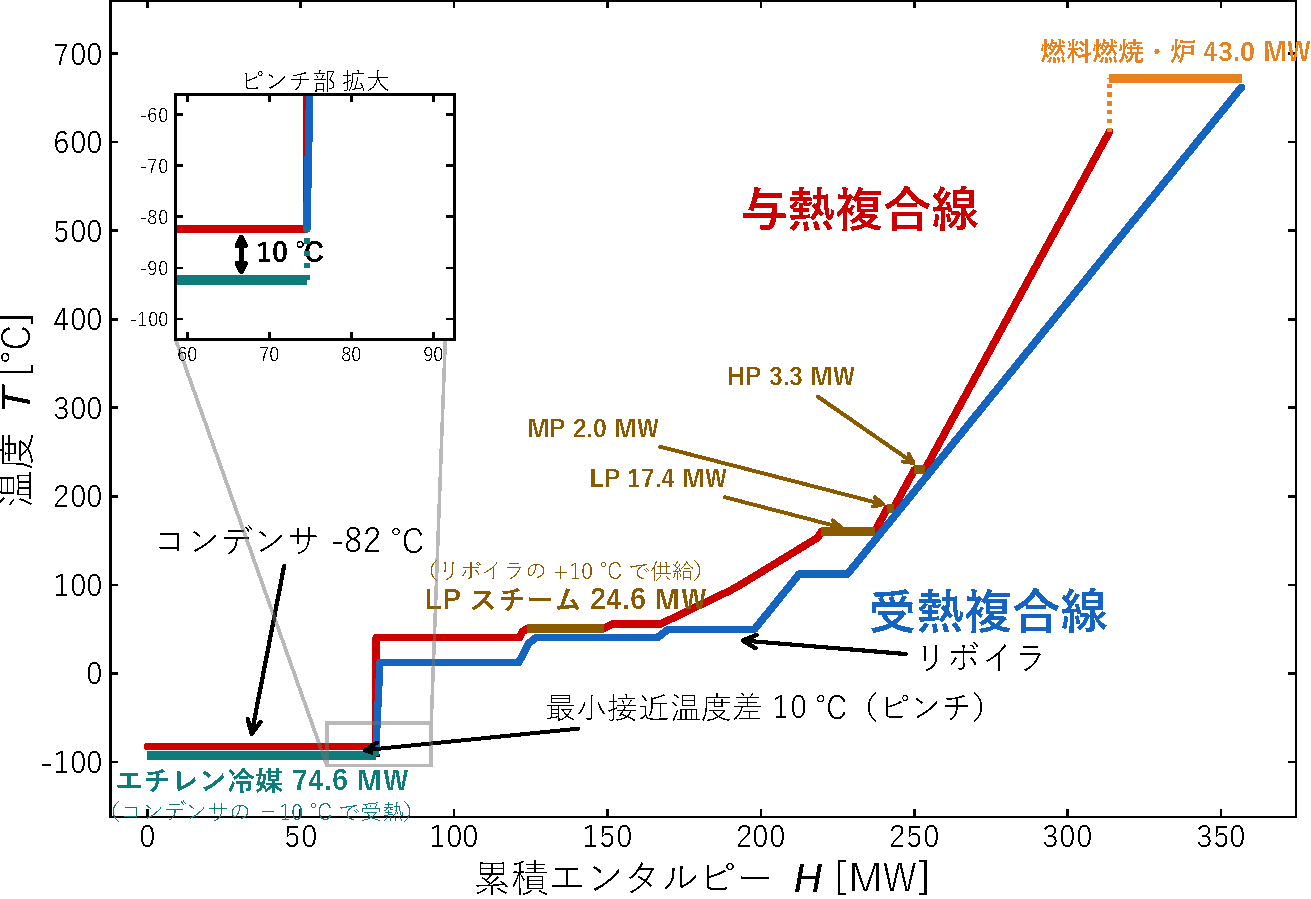
\includegraphics[width=\dimexpr\linewidth-2mm\relax]{composite_slide}
\end{frame}
}


\section{反応工程}
% =====================================================================
%  04  反応工程 — 反応ネットワーク・速度式・触媒失活
%  source_memo: 04_reaction.tex §4.2(反応ネットワークと速度式) /
%               §4.3.2-3(コーキングと活性低下 a(t,T))
%  失活グラフ実データ: pdh_simulator/src/catalyst_model.py _A_MATRIX
%               （要項§3-3 提供データ、温度400-700C × 時間0-30min）
%  方針：反応器モデル（支配方程式・Ergun）は載せない。
%        上=反応式と速度式／下左=触媒失活の要点／下右=a(t,T) グラフ。
%        色は反応式の化学種と、温度で意味を持つグラフの系列のみ。
% =====================================================================
% 活性 a を緑の太字で統一表示するマクロ
\definecolor{ActGreen}{HTML}{1BC24A}
\providecommand{\actA}{}\renewcommand{\actA}{{\color{ActGreen}\scalebox{1.2}{\ensuremath{\boldsymbol{a}}}}}
% 左カラム「触媒失活」見出し＋説明文を丸ごと左右に動かすつまみ。
% 正で右へ・負で左へ（0 で本文左マージン3mmのまま）。見出しと本文は連動して動く。ここの数字だけ変える。
\newlength{\descIndent}\setlength{\descIndent}{-2.8mm}
% 説明文の箱の幅。広げるほどグラフ左の余白を文章が使い、折り返しが減る。
\newlength{\descWidth}\setlength{\descWidth}{46mm}
% グラフ横幅を左から縮める量。大きいほどグラフが小さくなり、文章の余地が増える（右枠はスライド端のまま）。
\newlength{\grShrink}\setlength{\grShrink}{6mm}
\begin{frame}[t]

  \vspace*{0.6em}
  % ===== 上：反応ネットワーク + 速度式（全幅）======================
  {\normalsize
   \renewcommand{\arraystretch}{1.18}%
   \begin{tabular}{@{}l@{\hspace{0.7em}}l@{\hspace{0.6em}}l@{}}
     {\scriptsize 脱水素}
       & \setlength{\fboxsep}{4pt}\setlength{\fboxrule}{1.2pt}%
         \fcolorbox{HeaderBlue}{white}{\boldmath$\mathrm{C_3H_8 \rightleftharpoons {\color{SpRed}C_3H_6} + H_2}$}
       & $\displaystyle r_1 = \actA\,k_1\frac{p_{\mathrm{C_3H_8}} - p_{\mathrm{C_3H_6}}p_{\mathrm{H_2}}/K_{\mathrm{eq}}}{1 + p_{\mathrm{C_3H_6}}/K_B}$ \\
     {\scriptsize クラッキング} & {\boldmath$\mathrm{C_3H_8 \rightarrow {\color{SpBlue}C_2H_4} + CH_4}$}
       & $\displaystyle r_2 = k_2\,p_{\mathrm{C_3H_8}}$ \\
     {\scriptsize 水素化} & {\boldmath$\mathrm{{\color{SpBlue}C_2H_4} + H_2 \rightarrow {\color{SpBlue}C_2H_6}}$}
       & $\displaystyle r_3 = k_3\,p_{\mathrm{C_2H_4}}p_{\mathrm{H_2}}$ \\
     {\scriptsize コーキング} & {\boldmath$\mathrm{{\color{SpRed}C_3H_6} \rightarrow 3\,{\color{SpBlue}CH_{0.5}} + 2.25\,H_2}$}
       & {\scriptsize 物質収支では微量・触媒を失活} \\
   \end{tabular}}

  \vspace{0.12em}
  {\setlength{\fboxsep}{4pt}\setlength{\fboxrule}{0.8pt}%
   \noindent\fcolorbox{HeaderBlue}{white}{%
    \parbox{\dimexpr\linewidth-2\fboxsep-2\fboxrule\relax}{%
      \scriptsize 想定触媒：\textbf{\ce{Cr2O3}-\ce{Al2O3}}、主反応 \(\Delta H^{\circ}_{1}\approx +124\,\mathrm{kJ/mol}\)（吸熱）\par
      \vspace{2pt}
      速度定数は修正アレニウス、基準 $T_0=793\,\mathrm{K}$。$K_B$ はプロピレン吸着で高転化時 $r_1$ を抑制。}}}

  \vspace{0.35em}

  % ===== 下：触媒失活（左・簡潔）と a(t,T) グラフ（右・最大化）====
  %  方針：xラベルを yshift で目盛に密着、図タイトル・出典を負 vspace で詰めて
  %        運転時間の前後・タイトル/出典間の余白を最小化し、グラフ高さを最大化。
  \begin{columns}[T,onlytextwidth]
    \begin{column}{0.26\textwidth}
      \noindent\hspace*{\descIndent}\makebox[0pt][l]{\begin{minipage}[t]{\descWidth}
      \vspace*{1.0em}
      {\bfseries 触媒失活}\par
      \vspace{0.5em}
      {\footnotesize\raggedright\linespread{1.18}\selectfont
        コークが活性点を被覆し失活。\par
        \vspace{0.25em}
        活性 $\actA(t,T)$ は主反応 $r_1$ のみに作用\\
        （副反応には不作用）。\par
        \vspace{0.25em}
        運転温度では数分で大きく低下\par
        \quad $\to$\,\textbf{短周期の再生が不可欠}
      }
      \end{minipage}}
    \end{column}
    \begin{column}{0.74\textwidth}
      \noindent\hspace*{\dimexpr5.90mm+\grShrink\relax}\makebox[0pt][l]{%
      \begin{tikzpicture}
        \begin{axis}[
          font=\scriptsize,
          width=\dimexpr\linewidth-\grShrink\relax, height=5.08cm,
          xmin=0, xmax=30, ymin=0, ymax=1,
          enlarge x limits=false, enlarge y limits=false,
          xtick={0,10,20,30}, ytick={0,0.2,0.4,0.6,0.8,1.0},
          xlabel={運転時間 [min]}, ylabel={活性 $\actA$},
          xlabel near ticks, ylabel near ticks,
          x label style={yshift=2.55mm}, y label style={xshift=1.6mm},
          tick align=inside, xtick pos=both, ytick pos=both,
          legend style={font=\scriptsize, at={(0.985,0.98)}, anchor=north east,
                        draw=none, fill=white, fill opacity=0.7, text opacity=1,
                        inner sep=2pt, row sep=0.4pt},
          legend columns=1, legend cell align=left,
          no markers, line width=0.9pt,
        ]
          \addplot[blue]          coordinates {(0,1)(5,0.94)(10,0.90)(15,0.86)(20,0.84)(25,0.82)(30,0.81)}; \addlegendentry{$400\,^\circ$C}
          \addplot[cyan!70!blue]  coordinates {(0,1)(5,0.87)(10,0.80)(15,0.76)(20,0.72)(25,0.70)(30,0.68)}; \addlegendentry{$450\,^\circ$C}
          \addplot[teal]          coordinates {(0,1)(5,0.80)(10,0.68)(15,0.622)(20,0.57)(25,0.52)(30,0.49)}; \addlegendentry{$500\,^\circ$C}
          \addplot[olive]         coordinates {(0,1)(5,0.67)(10,0.52)(15,0.42)(20,0.36)(25,0.31)(30,0.28)}; \addlegendentry{$550\,^\circ$C}
          \addplot[orange]        coordinates {(0,1)(5,0.52)(10,0.35)(15,0.24)(20,0.18)(25,0.15)(30,0.13)}; \addlegendentry{$600\,^\circ$C}
          \addplot[red!70!black]  coordinates {(0,1)(5,0.38)(10,0.21)(15,0.13)(20,0.09)(25,0.07)(30,0.06)}; \addlegendentry{$650\,^\circ$C}
          \addplot[red]           coordinates {(0,1)(5,0.25)(10,0.12)(15,0.08)(20,0.06)(25,0.05)(30,0.04)}; \addlegendentry{$700\,^\circ$C}
          \node[font=\scriptsize\bfseries, anchor=north, fill=white, fill opacity=0.6,
                text opacity=1, inner sep=1.5pt] at (axis cs:10.5,0.985) {高温ほど急速に失活};
        \end{axis}
      \end{tikzpicture}}\par
      \centering
      \vspace*{-0.92em}
      {\scriptsize 　　　　　触媒活性 $\actA$ の経時低下（温度別）}\par
      \vspace*{-0.66em}
      {\tiny 速度式パラメータ・活性データの出典：第17回プロセスデザイン学生コンテスト要項}
    \end{column}
  \end{columns}

\end{frame}


\section{反応器設計}
% =====================================================================
%  06  反応器設計 — 左右2カラム
%  左：性質→部品マップ（上）＋形式選定3判断の表（下）
%  右：反応器の説明文（上・小さめ）＋浅床軸流・多基切替式固定床の模式図（下）
%  source_memo: report/chapters/04_reaction.tex §4.1 形式選定3判断 /
%               §4.4 接触時間 τ∝1/u² / 反応器概念断面 TikZ。
%  方針：[t] で帯直下から少し下げる。丸括弧禁止。はみ出し・重なりなし。
% =====================================================================
\begin{frame}[t]

  \vspace{0.35em}
  \begin{columns}[T,onlytextwidth]
    % ===== 左：性質→部品マップ（上）＋形式選定の3判断の表（下）=====
    \begin{column}{0.40\textwidth}
      \centering
      \resizebox{\linewidth}{!}{%
      \begin{tikzpicture}[
        >=Stealth, font=\small,
        prop/.style={draw=black!50, rounded corners=2pt, align=center,
                     inner sep=3pt, minimum height=0.7cm, text width=2.0cm},
        part/.style={draw=HeaderBlue, fill=HiBlue!45, rounded corners=2pt, align=center,
                     inner sep=3pt, minimum height=0.6cm, text width=2.9cm,
                     font=\small\bfseries},
        link/.style={-{Stealth[length=2mm]}, ArrowBlue, line width=1pt},
      ]
        \node[prop] (heat) at (0,2.85) {吸熱};
        \node[prop] (eq)   at (0,1.42){平衡支配\\$0.5$ bar};
        \node[prop] (coke) at (0,0)   {コーキング\\数分で失活};
        \node[part] (hgm)   at (3.7,2.85) {床内 HGM 補温};
        \node[part] (shal)  at (3.7,1.9)  {浅床軸流};
        \node[part] (multi) at (3.7,0.95) {多基・大断面・低速};
        \node[part] (swing) at (3.7,0.0)  {切替式　反応 $\rightleftarrows$ 再生};
        \draw[link] (heat.east) -- (hgm.west);
        \draw[link] (eq.east)   -- (shal.west);
        \draw[link] (eq.east)   -- (multi.west);
        \draw[link] (coke.east) -- (swing.west);
      \end{tikzpicture}}\par

      \vspace{1.0em}
      \raggedright
      {\small\bfseries 形式選定の3判断と採用根拠}\par
      \vspace{0.4em}
      {\scriptsize\renewcommand{\arraystretch}{1.15}%
       \begin{tabular}{@{}l l c@{}}
         \toprule
         判断 & 候補 & 採否 \\
         \midrule
         \multirow{2}{*}{触媒再生}
            & 移動床            & $\times$ \\
            & {\color{SpRed}並列切替固定床} & $\bigcirc$ \\
         \midrule
         \multirow{3}{*}{流通形式}
            & 軸流深床   & $\times$ \\
            & 径方向流   & $\triangle$ \\
            & {\color{SpRed}浅床軸流}   & $\bigcirc$ \\
         \midrule
         \multirow{2}{*}{熱補償}
            & 段間再加熱 & $\times$ \\
            & {\color{SpRed}床内 HGM}   & $\bigcirc$ \\
         \bottomrule
       \end{tabular}}\par
      \vspace{0.25em}
      {\tiny\raggedright $\times$ 移動床は失活追従不可、$\triangle$ 径方向流は機構複雑\par
       \vspace{0.18em}
       $\times$ 段間再加熱は床温を戻すのみで分単位の急速失活に間に合わない。切替再生で蓄えた熱を HGM が床内補償\par}
    \end{column}

    % ===== 右：反応器の特徴（上・小さめ）＋模式図（下）============
    \begin{column}{0.60\textwidth}
      % 特徴文：左のフロー図から離すため右へインデント、文字は小さめ
      \hspace*{9mm}\begin{minipage}{\dimexpr\linewidth-9mm\relax}
        \raggedright
        {\bfseries 反応器の特徴}\par
        \vspace{0.3em}
        {\scriptsize\raggedright\linespread{1.18}\selectfont
          ・\textbf{Catofin 型}の浅床軸流・多基切替式固定床を採用。\par
          ・吸熱反応と再生（コーク燃焼）を周期的に切替え、\textbf{計 14 基}で連続運転。\par
          ・床内の蓄熱体 \textbf{HGM} が反応熱を供給し床温を維持。\par
          ・大断面・低流速で接触時間を確保（$\tau\propto 1/u^{2}$、流速半減で 4 倍）し、短周期切替で失活に追従。\par
        }
      \end{minipage}\par

      \vspace{1.2em}   % 模式図を下げ、最下部をスライド下端に合わせる
      \centering
      {\bfseries\color{SpRed}浅床軸流・多基切替式固定床の模式図}\par
      \vspace{0.15em}
      \resizebox{0.95\linewidth}{!}{%
      \begin{tikzpicture}[
        >=Stealth,
        proc/.style={-{Stealth[length=2.4mm]}, line width=1.2pt},
        wall/.style={line width=1.3pt},
        lead/.style={line width=0.4pt, black!55},
        lbl/.style={font=\large, align=center},
      ]
        \foreach \dx/\toplab/\botlab/\stt/\bcol/\acol in {%
           0/{原料ガス}/{製品}/{反応中}/{ArrowBlue}/{ArrowBlue},
           5.4/{空気}/{燃焼ガス}/{再生中}/{orange!85!red}/{orange!85!red}%
        }{
          \begin{scope}[xshift=\dx cm]
            \def\R{1.72}\def\Hb{1.48}\def\ry{0.80}
            \draw[wall] (-\R,0)--(-\R,\Hb); \draw[wall] (\R,0)--(\R,\Hb);
            \draw[wall] (-\R,\Hb) arc[start angle=180, end angle=0, x radius=\R, y radius=\ry];
            \draw[wall] (\R,0) arc[start angle=0, end angle=-180, x radius=\R, y radius=\ry];
            \draw[line width=0.7pt] (-\R+0.07,\Hb-0.30)--(\R-0.07,\Hb-0.30);
            \fill[pattern=dots, pattern color=\bcol] (-\R+0.07,\Hb-0.80) rectangle (\R-0.07,\Hb-0.38);
            \draw[black!40] (-\R+0.07,\Hb-0.80) rectangle (\R-0.07,\Hb-0.38);
            \draw[line width=0.7pt] (-\R+0.07,\Hb-0.86)--(\R-0.07,\Hb-0.86);
            \draw[wall] (-0.17,\Hb+\ry-0.02)--(-0.17,\Hb+\ry+0.30);
            \draw[wall] (0.17,\Hb+\ry-0.02)--(0.17,\Hb+\ry+0.30);
            \draw[proc, \acol] (0,\Hb+\ry+0.92)--(0,\Hb+\ry+0.36);
            \node[lbl, above] at (0,\Hb+\ry+0.90) {\toplab};
            \draw[wall] (-0.17,-\ry+0.02)--(-0.17,-\ry-0.30);
            \draw[wall] (0.17,-\ry+0.02)--(0.17,-\ry-0.30);
            \draw[proc, \acol] (0,-\ry-0.36)--(0,-\ry-0.92);
            \node[lbl, below] at (0,-\ry-0.90) {\botlab};
            \node[font=\Large\bfseries, text=\acol] at (0,-\ry-1.74) {\stt};
          \end{scope}
        }
        \node[lbl, anchor=east, font=\scriptsize] (bl) at (-2.15,1.30) {触媒・HGM\\浅床};
        \draw[lead] (bl.east) -- (-1.60,1.00);
        \node[lbl, anchor=east, font=\scriptsize] (gl) at (-2.15,0.40) {支持グリッド};
        \draw[lead] (gl.east) -- (-1.60,0.62);
        \draw[{Stealth[length=2.6mm]}-{Stealth[length=2.6mm]}, line width=1.6pt, ArrowBlue]
              (1.95,0.95) -- (3.45,0.95);
        \node[lbl, ArrowBlue, font=\normalsize\bfseries, align=center] at (2.7,1.55) {周期\\切替};
        \node[font=\large, align=center, text=black] at (2.7,-3.45)
              {反応 $\rightleftarrows$ 再生 を周期交代　計 14 基};
      \end{tikzpicture}}
    \end{column}
  \end{columns}

\end{frame}


\section{反応器設計に用いた方程式}
% =====================================================================
%  07  支配方程式（ヘッダー＝支配方程式）
%  source_memo: 04_reaction.tex §4.2.4 支配方程式（物質・エネルギー・Ergun）/
%               §4.2.5 スイング設計（N_swing,sets・V_cat・N_parallel・V_vessel）/
%               §4.2 量論行列(eq:stoich_matrix)・成分ベクトル
%  方針：見出しは小チップ。速度式は §反応工程で既出のため載せない。
%        各列に「式（上）＋記号表（下）」を縦積みし、中央を全高の縦線で仕切る。
%        左＝モデル（式＋記号表：ベクトル/行列 F・r・ν・ΔH・Cp を収録）。
%        右＝スイング設計（式＋記号表）。表は 1記号=1行・2群・群間に縦罫線。
%        モデル式は短いので左表を直下から始め余白を回収し表を最大化。色なし・丸括弧禁止。
% =====================================================================
\begin{frame}[t]

  \vspace{0.15em}

  \begin{columns}[T,onlytextwidth]
    % ===== 左：モデル（式＋記号表）================================
    \begin{column}{0.49\textwidth}
      \fbox{\scriptsize モデル}\par
      \vspace{0.75em}
      {\fontsize{5.5}{6.6}\selectfont [物質収支]}\par
      {\centering$\displaystyle\frac{d\boldsymbol{F}}{dz}=(1-\varepsilon)\,A_{\mathrm{cross}}\,\boldsymbol{\nu}\,\boldsymbol{r}$\par}
      \vspace{0.95em}
      {\fontsize{5.5}{6.6}\selectfont [エネルギー収支・断熱]}\par
      {\centering$\displaystyle\frac{dT}{dz}=-\frac{(1-\varepsilon)\,A_{\mathrm{cross}}\,\boldsymbol{\Delta H}^{\!\top}\boldsymbol{r}}{\boldsymbol{F}^{\!\top}\boldsymbol{C}_p}$\par}
      \vspace{0.95em}
      {\fontsize{5.5}{6.6}\selectfont [Ergun]}\par
      {\centering\resizebox{\linewidth}{!}{$\displaystyle\frac{dP}{dz}=-\Big[\,150\frac{(1-\varepsilon_b)^2\mu u}{\varepsilon_b^3(\phi d_p)^2}
           +1.75\frac{(1-\varepsilon_b)\rho u^2}{\varepsilon_b^3\phi d_p}\,\Big]$}\par}
      \vspace{0.6em}
      {\color{black!25}\rule{\linewidth}{0.4pt}}\par
      \vspace{0.45em}
      % --- 左表：モデルの記号（ベクトル/行列＋支配式スカラー）2群 ---
      \resizebox{\linewidth}{!}{%
       \renewcommand{\arraystretch}{1.25}%
       \begin{tabular}{@{}l l l @{\hspace{1em}}|@{\hspace{1em}} l l l@{}}
         \toprule
         $\boldsymbol{F}$        & モル流量 & mol/s
           & $\varepsilon_b$ & 粒子間空隙率 & -- \\
         $\boldsymbol{r}$        & 反応速度 & mol/m$^3$s
           & $d_p$          & 粒径          & m \\
         $\boldsymbol{\nu}$      & 量論行列 & --
           & $\phi$          & 形状係数      & -- \\
         $\boldsymbol{\Delta H}$ & 反応熱   & kJ/mol
           & $T$            & 温度          & K \\
         $\boldsymbol{C}_p$      & 熱容量   & J/molK
           & $P$            & 全圧          & Pa \\
         $z$                     & 軸位置   & m
           & $u$            & 空塔速度      & m/s \\
         $A_{\mathrm{cross}}$    & 断面積   & m$^2$
           & $\rho$          & 密度          & kg/m$^3$ \\
         $\varepsilon$           & 床/容器体積比 & --
           & $\mu$          & 粘度          & Pa$\cdot$s \\
         \bottomrule
       \end{tabular}}
    \end{column}

    % ===== 中央：全高の仕切り線 ==================================
    \begin{column}{0.02\textwidth}
      \centering
      {\color{black!35}\rule[-6.9cm]{0.6pt}{7.05cm}}
    \end{column}

    % ===== 右：スイング設計（式＋記号表）==========================
    \begin{column}{0.49\textwidth}
      \fbox{\scriptsize スイング設計}\par
      \vspace{0.45em}
      {\fontsize{5.5}{6.6}\selectfont [再生追従のセット数]}\par
      {\centering$\displaystyle N_{\mathrm{swing,sets}}=\left\lceil\frac{t_{\mathrm{regen}}}{t_{\mathrm{cyc}}}\right\rceil+1$\par}
      \vspace{0.35em}
      {\fontsize{5.5}{6.6}\selectfont [触媒体積]}\par
      {\centering$\displaystyle V_{\mathrm{cat}}=(1-\varepsilon)\,z_{\mathrm{cat}}\,\frac{\pi D^2}{4}$\par}
      \vspace{0.35em}
      {\fontsize{5.5}{6.6}\selectfont [容器分割の並列基数]}\par
      {\centering$\displaystyle N_{\mathrm{parallel}}=\max\!\left(\left\lceil\frac{V_{\mathrm{cat}}}{V_{\mathrm{cat,max}}}\right\rceil,\,1\right)$\par}
      \vspace{0.35em}
      {\fontsize{5.5}{6.6}\selectfont [容器1基の体積　CAPEX 基準]}\par
      {\centering$\displaystyle V_{\mathrm{vessel}}=\frac{z_{\mathrm{cat}}}{N_{\mathrm{parallel}}}\cdot\frac{\pi D^2}{4}$\par}
      \vspace{0.5em}
      {\color{black!25}\rule{\linewidth}{0.4pt}}\par
      \vspace{0.4em}
      % --- 右表：スイング設計の記号 2群 ---
      \resizebox{\linewidth}{!}{%
       \renewcommand{\arraystretch}{1.25}%
       \begin{tabular}{@{}l l l @{\hspace{1em}}|@{\hspace{1em}} l l l@{}}
         \toprule
         $z_{\mathrm{cat}}$   & 触媒層長 & m
           & $V_{\mathrm{cat}}$    & 触媒体積       & m$^3$ \\
         $D$                  & 内径     & m
           & $V_{\mathrm{vessel}}$ & 容器体積       & m$^3$ \\
         $t_{\mathrm{cyc}}$   & 反応時間 & s
           & $V_{\mathrm{cat,max}}$ & 最大触媒体積  & m$^3$ \\
         $t_{\mathrm{regen}}$ & 再生時間 & s
           & $N_{\mathrm{parallel}}$ & 並列基数     & -- \\
         & & & $N_{\mathrm{swing,sets}}$ & スイングセット数 & -- \\
         \bottomrule
       \end{tabular}}
    \end{column}
  \end{columns}

\end{frame}


\section{浅床軸流・多基スイング反応器}
% =====================================================================
%  08  反応器プロファイル — 炉内 軸方向挙動＋検証諸元
%  source_memo: monitor/reactor_axial_profile.ipynb 出力
%               reactor_axial_TX.png / reactor_axial_selectivity.png、
%               §4.x 検証諸元 Table reactor_verification（trial #201）
%  方針：左=軸方向プロファイル2図（T/X のHGM補償効果・選択率の床内崩落）、
%        右=検証諸元。丸括弧禁止。
% =====================================================================
\begin{frame}

  \begin{columns}[T,onlytextwidth]
    % ===== 左：軸方向プロファイル =================================
    \begin{column}{0.6\textwidth}
      {\bfseries HGM 補償が床温を維持し転化率を伸ばす}\par
      \vspace{0.1em}
      \centering
      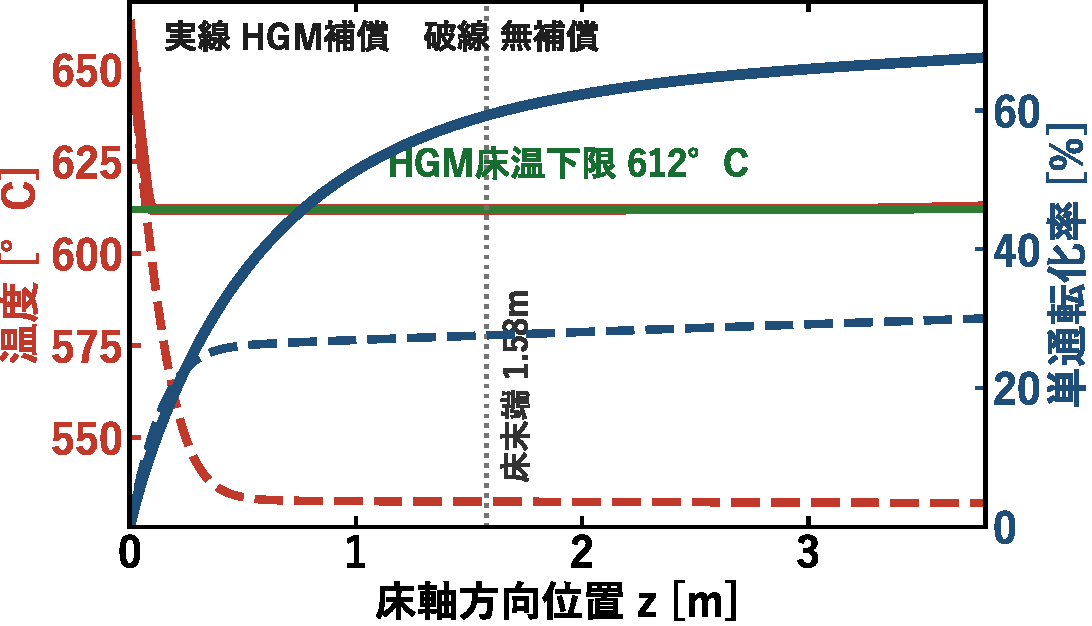
\includegraphics[width=0.78\linewidth]{reactor_axial_TX}\par
      \vspace{0.2em}
      {\bfseries 選択率は床後半で崩落し出口値へ収束}\par
      \vspace{0.1em}
      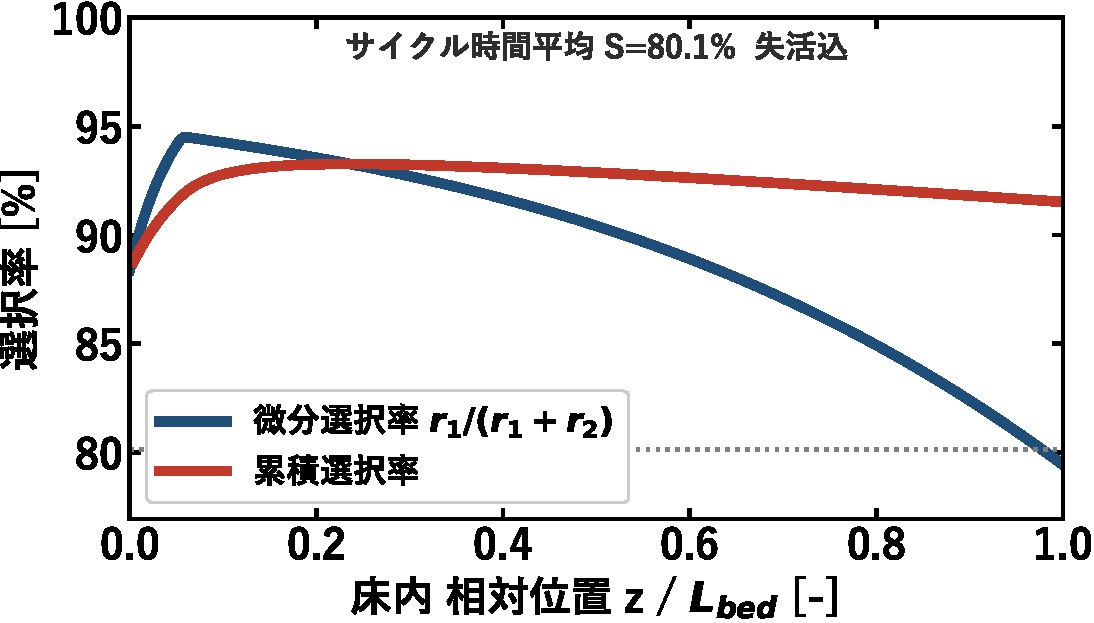
\includegraphics[width=0.78\linewidth]{reactor_axial_selectivity}\par
    \end{column}

    % ===== 右：検証諸元（trial #125）=============================
    \begin{column}{0.4\textwidth}
      {\bfseries 検証諸元　{\scriptsize 最良設計点}}\par
      \vspace{0.5em}
      {\setlength{\fboxsep}{5pt}\setlength{\fboxrule}{1pt}%
       \fcolorbox{HeaderBlue}{white}{%
        \footnotesize\renewcommand{\arraystretch}{1.25}%
        \begin{tabular}{@{}l@{\hspace{0.8em}}r@{}}
          入口温度 $T_{\mathrm{in}}$   & $935$ K \\
          出口温度 $T_{\mathrm{out}}$  & $885$ K \\
          床温降下 $\Delta T$          & $50$ K \\
          転化率 $X$                   & $40.6\,\%$ \\
          選択率 $S$                   & $80.1\,\%$ \\
          浅床厚 $L_{\mathrm{bed}}$    & $1.58$ m \\
          触媒粒径 $d_p$               & $5.84$ mm \\
          床 $\Delta P/P$              & $1.7\,\%$ \\
          総 $\Delta P/P$              & $3.3\,\%$ \\
          総基数 $N_{\mathrm{total}}$  & $14$ 基 \\
        \end{tabular}}}\par
      \vspace{0.8em}
      {\scriptsize 図の $T$・$X$ は新触媒断面、\par
       転化率 $40.6\,\%$・選択率 $80.1\,\%$ は\par
       失活を含むサイクル時間平均。\par
       無補償では床温が下限へ張り付き\par
       転化率が頭打ちとなる。}\par
    \end{column}
  \end{columns}

\end{frame}


\section{反応器分析}
% =====================================================================
%  09  転化率の天井（断熱平衡）と熱補償 HGM・リサイクルの必然性（旧08、反応器プロファイルと順序入替）
%  ※ ヘッダーは main.tex の \section{転化率の天井} で設定。
%  source_memo: 04_reaction.tex §4.6 単通転化率と選択率の上限（断熱平衡の天井）/
%               §4.7 反応熱の補償方式（HGM）。図 reactor_xt_slide（figures/make_reactor_xt_slide.py）。
%               数値：ΔH1≈+124 kJ/mol、断熱平衡 524℃・23%、等温保持 78%、Q_HGM=24.96 MW（trial #201）。
%  方針：8(プロファイル)の後に「なぜHGMが要るか」を置く。
%        左＝問題（断熱の頭打ち）→打破（HGM→接触時間→リサイクル）、右＝X–T線図。
%        丸括弧禁止・色は天井の数値のみ赤。
% =====================================================================
\begin{frame}[t]

  \vspace{0.2em}

  \begin{columns}[T,onlytextwidth]
    % ===== 左：三段でまとめる（転化率の天井／打破＝多段 vs HGM／選択率の天井）===
    \begin{column}{0.53\textwidth}
      {\bfseries 転化率の天井}\par
      \vspace{0.35em}
      {\footnotesize
       ・強吸熱の自己冷却で断熱平衡に頭打ち\par
       \hspace{1em}断熱 {\color{SpRed}\textbf{23\,\%}}　$\Leftrightarrow$　等温保持 78\,\%\par
       ・触媒を増やしても破れない　律速は平衡\par
      }
      \vspace{1.0em}
      {\bfseries 天井の打破は二択}\par
      \vspace{0.35em}
      {\footnotesize
       ・多段直列＋段間再加熱で各段の平衡をリセット\par
       \hspace{1em}この方式は反応器が \textbf{3〜4 段}になる\par
       ・本設計は床内 HGM で床温維持・段間炉なし\par
       \hspace{1em}$\to$ 律速が接触時間へ　低速・多基で稼ぐ\par
       \hspace{1em}維持温度の平衡が上限 $\to$ \textbf{リサイクル必須}\par
      }
      \vspace{1.0em}
      {\bfseries 選択率の天井}\par
      \vspace{0.35em}
      {\footnotesize
       ・平衡近傍で微分選択率が崩落 $\to$ 積分 {\color{SpRed}\textbf{約 80\,\%}}\par
       ・固有上限 $S_{\max}=k_1/(k_1+k_2)$ は温度のみ\par
       \hspace{1em}$520\,^\circ$C で $99$\,\% ／ $750\,^\circ$C で $77$\,\%\par
      }
    \end{column}

    % ===== 右：断熱 X–T 線図（縦中央寄せ・キャプション無し）======
    \begin{column}{0.46\textwidth}
      \centering
      \vspace{2.8em}
      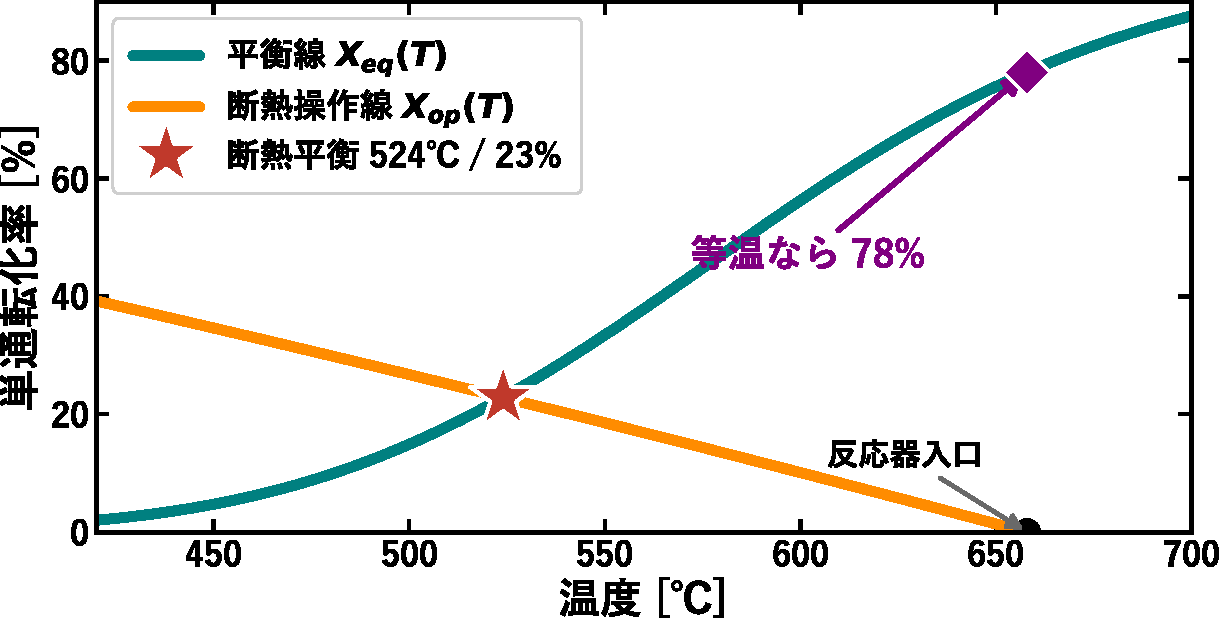
\includegraphics[width=\linewidth]{reactor_xt_slide}\par
    \end{column}
  \end{columns}

\end{frame}


\section{分離戦略}
% =====================================================================
%  10  分離戦略 — 左=分離の考え方（タイトル付き説明＋沸点マップ）｜右=工程フロー＋膜有無比較
%  source_memo: trial #201・07章 Table7.1/Fig7.1。分離目標(要求純度)を主役に:
%   C3H6 99.5wt%(α≈1.07)・H2 99.9mol%。脱ブタン=C4除去、脱エタン=軽質分離。
%   膜有無比較(共通フィード C3H6 60.7mol%): 膜+塔 TAC135/117段/94m vs 塔単独 TAC1625/200段/156m。
%  方針：まず左で「沸点→分離操作」の考え方を示し、右で工程フローと膜の効果へ。
%        左右は全高の仕切りで分ける。重なり・はみ出し・無駄余白なし。丸括弧禁止。
% =====================================================================
\definecolor{SepGreen}{HTML}{2E9E5B}
\begin{frame}[t]

  \vspace{0.05em}

  \begin{columns}[T,onlytextwidth]
    % ===== 左：分離の考え方（タイトル付き説明＋沸点マップ）｜右端に全高の仕切り =====
    \begin{column}{0.34\textwidth}
      \resizebox{!}{\dimexpr\textheight-6mm\relax}{%
      \begin{tikzpicture}[
        x=1cm, y=1cm, >=Stealth, font=\small,
        cut/.style={dashed, HeaderBlue, line width=0.8pt, -{Stealth[length=2mm]}},
        cuthard/.style={dashed, SpRed, line width=1.1pt, -{Stealth[length=2.2mm]}},
        tick/.style={HeaderBlue, line width=0.8pt},
        lab/.style={anchor=west, font=\small\bfseries},
        cmp/.style={anchor=west, font=\small},
        val/.style={anchor=east, font=\footnotesize, text=black!55},
      ]
        \useasboundingbox (-0.7,-0.9) rectangle (4.55,10.7);
        % --- 全高の仕切り縦線（右端：右の工程と分ける）---
        \draw[black!35, line width=0.9pt] (4.35,-0.8) -- (4.35,10.6);
        % --- タイトル付き説明 ---
        \node[anchor=north west, font=\large\bfseries, text=HeaderBlue] at (-0.6,10.5) {分離の考え方};
        \node[anchor=north west, font=\normalsize, text width=4.6cm, align=left] at (-0.6,9.7)
          {成分を沸点順に並べ、各境界に分離操作を割り当てた。沸点差の大きい境界は蒸留、沸点差 $6$ K と小さい C3 対のみ膜＋蒸留で分離。};
        % --- 沸点マップ（軸＝上が高沸点）---
        \draw[HeaderBlue, line width=1.3pt, ->] (0.3,0.5) -- (0.3,7.15);
        \node[anchor=west, font=\footnotesize, text=black!60] at (0.5,6.98) {[$^\circ$C]};
        \foreach \y/\name/\bp in {6.7/{$\mathrm{C_4H_{10}}$}/{$-1$}, 3.9/{$\mathrm{C_2H_6}$}/{$-89$}, 2.6/{$\mathrm{CH_4}$}/{$-161$}, 1.0/{$\mathrm{H_2}$}/{$-253$}}{
          \draw[tick] (0.15,\y) -- (0.45,\y);
          \node[cmp] at (0.5,\y) {\name};
          \node[val] at (0.0,\y) {\bp};
        }
        % C3 ペア（赤・近接）
        \draw[tick, SpRed] (0.15,5.5) -- (0.45,5.5);
        \draw[tick, SpRed] (0.15,5.1) -- (0.45,5.1);
        \node[cmp, text=SpRed] at (0.5,5.5) {$\mathrm{C_3H_8}$};
        \node[cmp, text=SpRed] at (0.5,5.1) {$\mathrm{C_3H_6}$};
        \node[val, text=SpRed] at (0.0,5.5) {$-42$};
        \node[val, text=SpRed] at (0.0,5.1) {$-48$};
        % cuts（境界ごとの分離操作）
        \draw[cut] (0.3,6.1) -- (1.9,6.1);
        \node[lab] at (2.0,6.1) {脱ブタン};
        \draw[cuthard] (0.3,5.3) -- (1.9,5.3);
        \node[lab, text=SpRed] at (2.0,5.3) {膜＋蒸留};
        \node[anchor=west, font=\footnotesize, text=SpRed] at (2.0,4.9) {沸点差 6 K};
        \draw[cut] (0.3,4.5) -- (1.9,4.5);
        \node[lab] at (2.0,4.5) {脱エタン};
        \draw[cut] (0.3,1.8) -- (1.9,1.8);
        \node[lab] at (2.0,1.8) {PSA};
        % --- マップのタイトル（最下部）---
        \node[anchor=north, font=\large\bfseries] at (1.8,-0.15) {沸点と分離操作};
      \end{tikzpicture}}
    \end{column}

    % ===== 右：工程フロー（上）＋膜有無の比較（下）=====
    \begin{column}{0.63\textwidth}
      % --- 上：横向き工程フロー（分離ブロックを緑・大きく強調）---
      \resizebox{\linewidth}{!}{%
      \begin{tikzpicture}[
        x=1cm, y=1cm, >=Stealth, font=\small,
        sep/.style={draw=SepGreen, line width=1.4pt, fill=SepGreen!22, rounded corners=3pt, align=center,
                    inner sep=2pt, minimum width=1.75cm, minimum height=1.05cm, font=\normalsize\bfseries},
        rxn/.style={draw=black, fill=white, rounded corners=2pt, align=center,
                    inner sep=2pt, minimum width=1.3cm, minimum height=0.72cm, font=\small\bfseries},
        raw/.style={align=center, font=\small\bfseries},
        goalC/.style={draw=SpRed, line width=1.2pt, fill=SpRed!12, rounded corners=3pt,
                      align=center, inner sep=4pt, text=SpRed},
        goalH/.style={draw=HeaderBlue, line width=1.2pt, fill=HiBlue!55, rounded corners=3pt,
                      align=center, inner sep=4pt},
        sub/.style={align=center, font=\scriptsize, text=black!60},
        main/.style={-{Stealth[length=2.8mm]}, HeaderBlue, line width=1.6pt},
        br/.style={-{Stealth[length=2.2mm]}, black!70, line width=1.1pt},
      ]
        % 主フロー（分離=緑で大きく、反応器=小さめ青）
        \node[raw] (raw) at (0.0,3.0) {原料\\LPG};
        \node[sep] (deb) at (2.0,3.0) {脱ブタン};
        \node[rxn] (rx)  at (4.0,3.0) {反応器};
        \node[sep] (de)  at (6.0,3.0) {脱エタン};
        \node[sep] (mc)  at (8.1,3.0) {膜＋蒸留};
        \node[goalC] (prod) at (10.8,3.0)
          {$\mathrm{C_3H_6}\!\mid\!\mathrm{C_3H_8}$\\[1pt]{\Large\bfseries 99.5 wt\%}};
        \draw[main] (raw) -- (deb);
        \draw[main] (deb) -- (rx);
        \draw[main] (rx) -- (de);
        \draw[main] (de) -- (mc);
        \draw[main] (mc) -- (prod);
        % PSA 枝（上）＋ H2 目標
        \node[sep, minimum width=1.3cm] (psa) at (6.0,5.2) {PSA};
        \draw[br] (de.north) -- node[left, font=\scriptsize]{軽質} (psa.south);
        \node[goalH] (h2) at (8.5,5.2)
          {$\mathrm{H_2}\!\mid\!$軽質\\[1pt]{\Large\bfseries 99.9 mol\%}};
        \draw[br] (psa.east) -- (h2.west);
        % 除去・循環（下、補助）
        \node[sub] (c4) at (2.0,1.35) {$\mathrm{C_4}$ 除去};
        \draw[br, black!55] (deb.south) -- (c4.north);
        \node[sub] (rec) at (8.1,1.35) {$\mathrm{C_3H_8}$ 循環};
        \draw[br, black!55] (mc.south) -- (rec.north);
      \end{tikzpicture}}

      \vspace{0.1em}

      % --- 下：膜有無の比較（レポート Fig7.1 形式のままスライド用に拡大）---
      \centering
      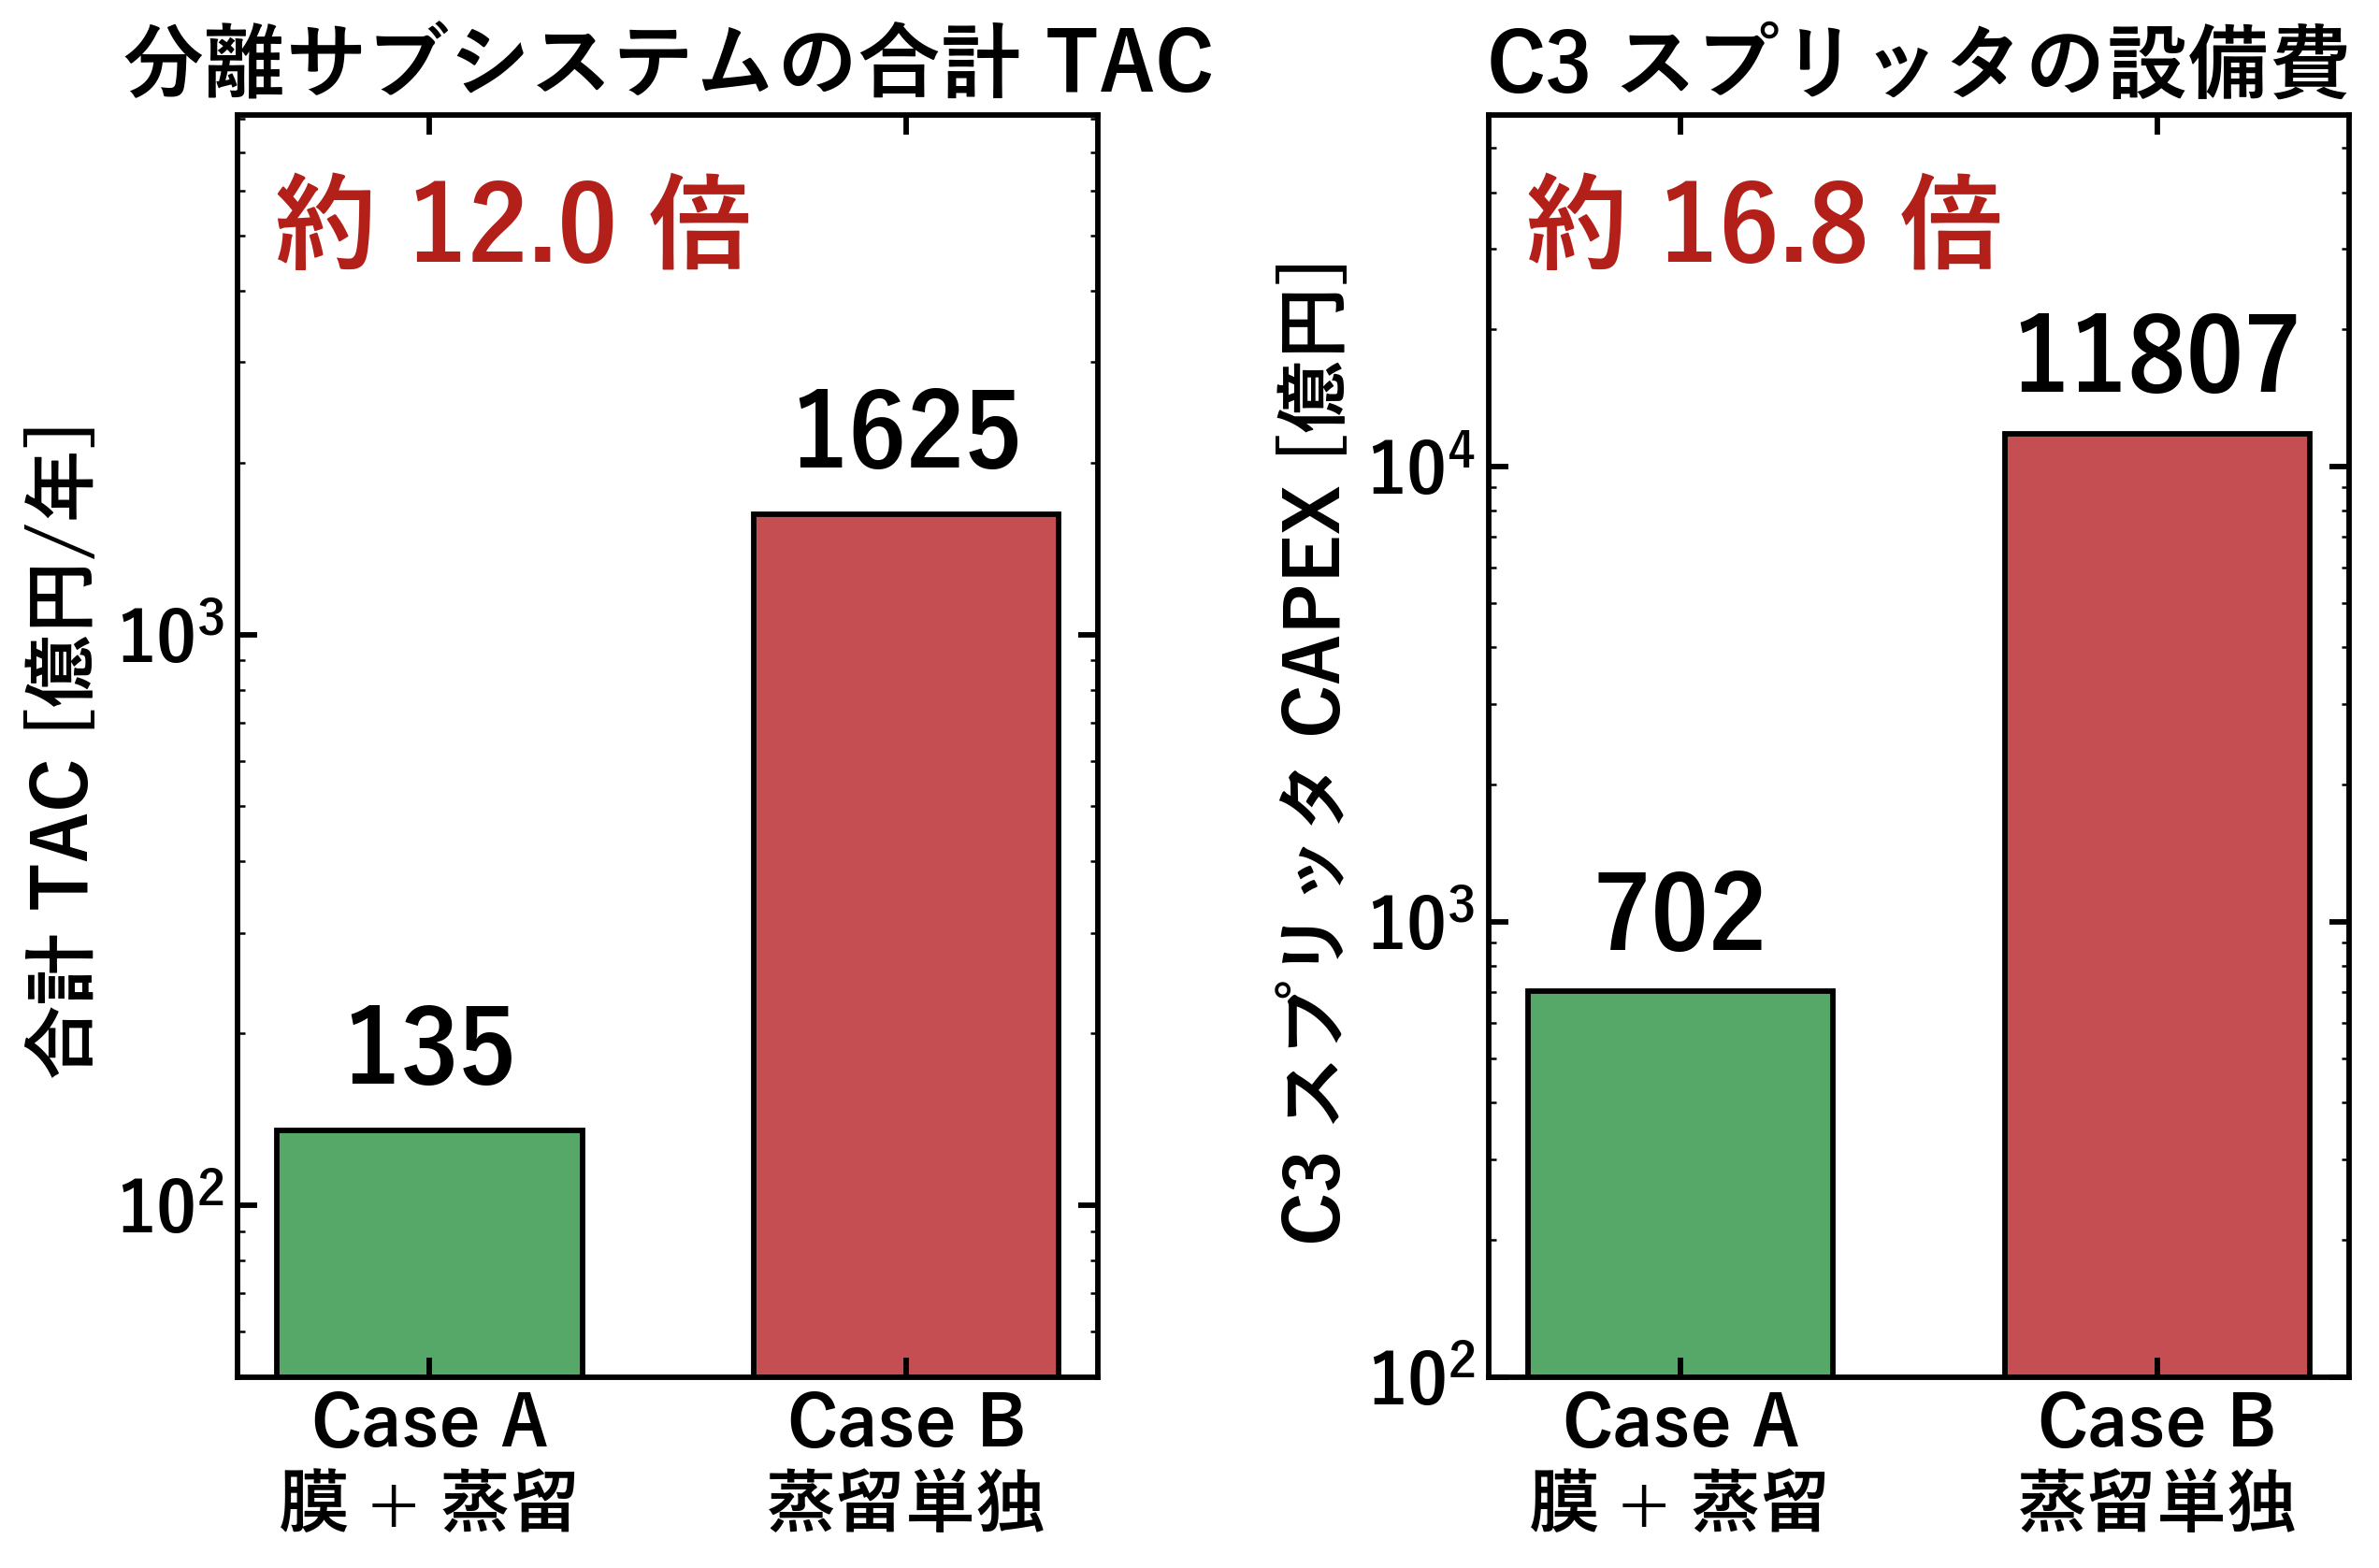
\includegraphics[width=\linewidth]{membrane_vs_dist3_slide}\par
      \vspace{0.08em}
      \raggedright
      {\scriptsize 膜無しは塔単独で $200$ 段・塔高 $156$ m を要する。}
    \end{column}
  \end{columns}

\end{frame}


\section{蒸留分離}
% =====================================================================
%  11  蒸留塔設計 — 左上=諸元表／右上=実寸比タワー図／下は空ける
%  source_memo: 05/06/07章＋trial #201。脱ブタン C3H8/C4H10 36段33m P19.5 全凝縮 α大／
%   脱エタン C2H6/C3H8 61段52m P7.9 部分凝縮 α3.9／C3 C3H6/C3H8 117段94m P16.7 全凝縮 α1.07(最難)。
%  方針：タイトル・共通設計枠組み・モデル名(SM/HYSYS)は載せない。表(左上)＋実寸比タワー(右上)。
%   下半分は意図的に空ける(後で別要素)。色は最難C3の赤のみ。丸括弧禁止。
% =====================================================================
\begin{frame}[t]

  \vspace{-0.7em}

  \begin{columns}[T,onlytextwidth]
    % ===== 左上：諸元表（SM/HYSYS は載せない／塔高は図側）=========
    \begin{column}{0.64\textwidth}
      {\scriptsize
       \setlength{\tabcolsep}{3pt}\renewcommand{\arraystretch}{1.04}%
       \begin{tabular}{@{}l c c c@{}}
         \toprule
          & 脱ブタン塔 & 脱エタン塔 & {\color{SpRed}C3 スプリッタ} \\
         \midrule
         軽／重キー & $\mathrm{C_3H_8}/\mathrm{C_4H_{10}}$ & $\mathrm{C_2H_6}/\mathrm{C_3H_8}$ & {\color{SpRed}$\mathrm{C_3H_6}/\mathrm{C_3H_8}$} \\
         塔頂留分 & $\mathrm{C_3H_8}$ & \begin{tabular}[t]{@{}c@{}}$\mathrm{H_2}\!\cdot\!\mathrm{CH_4}$\\[1pt]$\mathrm{C_2H_4}\!\cdot\!\mathrm{C_2H_6}$\end{tabular} & {\color{SpRed}$\mathrm{C_3H_6}$} \\
         比揮発度 $\alpha$ & 大 & $\approx 3.9$ & {\color{SpRed}\boldmath$\approx 1.07$} \\
         操作圧力 [bar] & $19.5$ & $7.9$ & {\color{SpRed}$16.7$} \\
         理論段数 & $36$ & $61$ & {\color{SpRed}\boldmath$117$} \\
         塔径 [m] & $4.0$ & $5.9$ & {\color{SpRed}$7.4$} \\
         還流比 & $2.0$ & $11.8$ & {\color{SpRed}$12.0$} \\
         フィード段 & $28$ & $31$ & {\color{SpRed}$96$} \\
         凝縮器 & 全凝縮 & 部分凝縮 & {\color{SpRed}全凝縮} \\
         リボイラ [MW] & $15.6$ & $44.2$ & {\color{SpRed}\boldmath$60.8$} \\
         \bottomrule
       \end{tabular}}
    \end{column}

    % ===== 右上：実寸比タワー図（名前＋塔高のみ）=================
    \begin{column}{0.36\textwidth}
      \centering
      \begin{tikzpicture}[
        x=1cm, y=1cm, >=Stealth, font=\scriptsize,
        name/.style={align=center, font=\scriptsize\bfseries},
        nameR/.style={align=center, font=\scriptsize\bfseries, text=SpRed},
      ]
        % 幅は塔径 D[m] に比例（4.0/5.9/7.4）、高さは塔高に比例（33/52/94m）
        % 脱ブタン D4.0 H33m
        \def\hB{1.34}\def\cB{0.55}\def\wB{0.33}
        \fill[pattern=horizontal lines, pattern color=HeaderBlue!55] (\cB-\wB,0) rectangle (\cB+\wB,\hB);
        \draw[HeaderBlue, line width=1pt] (\cB-\wB,0) rectangle (\cB+\wB,\hB);
        \node[name, anchor=south] at (\cB,\hB+0.06) {脱ブタン\\$33$ m};
        % 脱エタン D5.9 H52m
        \def\hE{2.11}\def\cE{1.9}\def\wE{0.49}
        \fill[pattern=horizontal lines, pattern color=HeaderBlue!55] (\cE-\wE,0) rectangle (\cE+\wE,\hE);
        \draw[HeaderBlue, line width=1pt] (\cE-\wE,0) rectangle (\cE+\wE,\hE);
        \node[name, anchor=south] at (\cE,\hE+0.06) {脱エタン\\$52$ m};
        % C3 D7.4 H94m（最難・赤）
        \def\hC{3.81}\def\cC{3.25}\def\wC{0.61}
        \fill[pattern=horizontal lines, pattern color=SpRed!50] (\cC-\wC,0) rectangle (\cC+\wC,\hC);
        \draw[SpRed, line width=1.2pt] (\cC-\wC,0) rectangle (\cC+\wC,\hC);
        \node[nameR, anchor=south] at (\cC,\hC+0.06) {C3 スプリッタ\\$94$ m};
        % 基準線＋注記
        \draw[black!35, line width=0.5pt] (\cB-0.5,0) -- (\cC+\wC+0.2,0);
      \end{tikzpicture}
    \end{column}
  \end{columns}

  \vspace{0.1em}

  % ===== 下：3塔の段プロファイル（組成・温度）全幅 =====
  \centering
  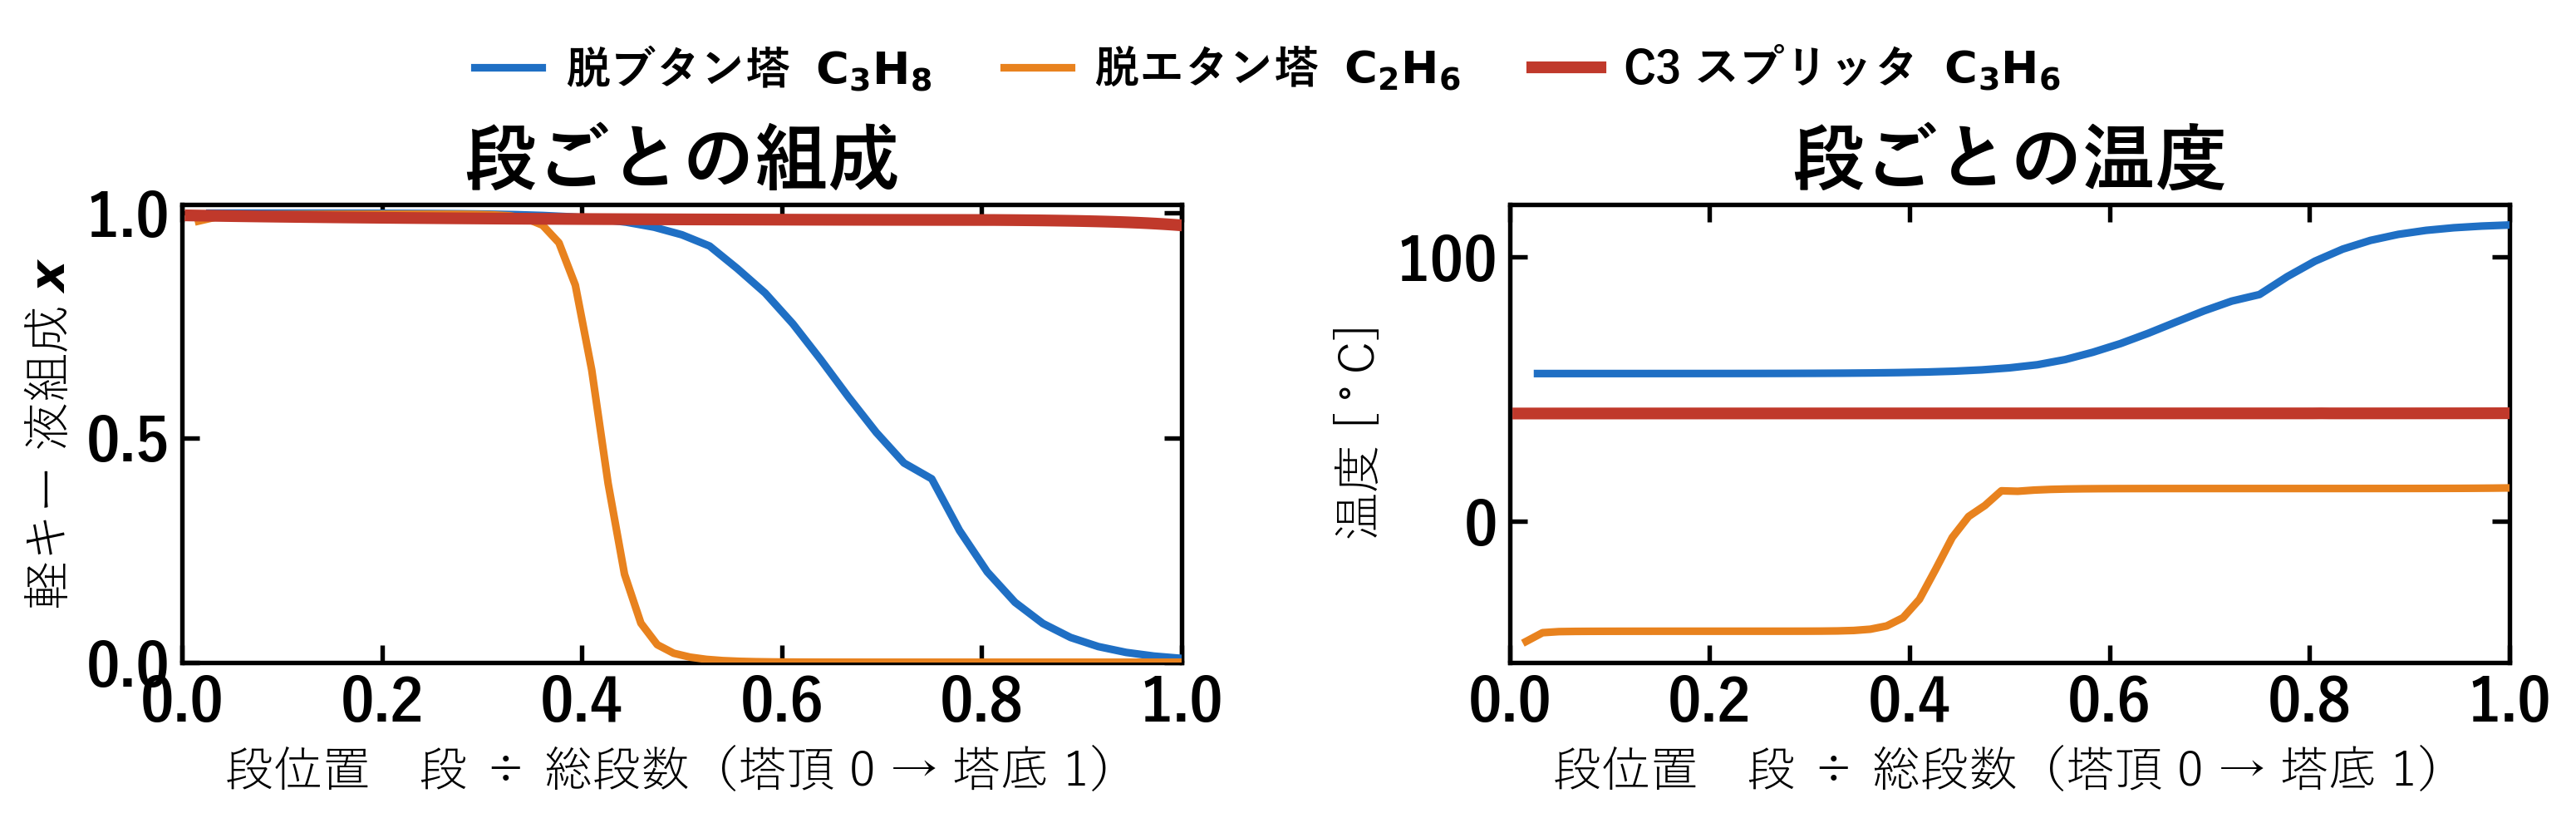
\includegraphics[width=0.97\linewidth]{dist_profiles}\par
  \vspace{0.12em}
  {\footnotesize\raggedright
   {\color{ArrowBlue}\textbf{脱ブタン}}・{\color{DipeOrange}\textbf{脱エタン}}：少ない段で組成・温度が急変化 ＝ 沸点差が大きく分離容易\par
   {\color{SpRed}\textbf{C3 スプリッタ}}：$117$ 段でも組成・温度ほぼ一定 ＝ 沸点差 $6$ K・$\alpha\!\approx\!1.07$ で分離困難\par}

\end{frame}


\section{膜分離}
% =====================================================================
%  12  プロピレン精製 — 膜ユニット（2段：上=概念図/プロファイル、下=表/膜選定）
%  source_memo: 07章＋top1_trial201.txt[Membrane]＋Hua et al. ACS AMI 2024,16,15273.
%   ZIF-8細孔4.0-4.2Å。多結晶ZIF-8膜 SF~300/52GPU(大面積化・高コスト難)。ポリマー膜=トレードオフ・可塑化。
%   ZIF-8 混合マトリックス膜(添加剤併用in-situ形成): 無添加57.7/22.5・最高222.5/10.1・頑健量産版74.9/26.6GPU。採用α90/40=楽観側。
%  方針：図で一目＋口頭。膜=緑SepGreen。丸括弧禁止。余白を作らず最下部まで使う。
% =====================================================================
\definecolor{SepGreen}{HTML}{2E9E5B}
\definecolor{DipeOrange}{HTML}{E8821E}
\begin{frame}[t]

  \vspace{0.1em}

  % ===== 上段：膜分離器の概念図（左）／膜面積プロファイル（右）=====
  \begin{columns}[T,onlytextwidth]
    \begin{column}{0.45\textwidth}
      \raggedright
      {\footnotesize\bfseries\color{SepGreen!45!black} 膜分離器}\par
      \vspace{0.4em}
      \resizebox{\linewidth}{!}{%
      \begin{tikzpicture}[
        x=1cm, y=1cm, >=Stealth, font=\Large,
        c6/.style={circle, fill=SepGreen, draw=black, line width=0.4pt, minimum size=4mm, inner sep=0},
        c8/.style={circle, fill=DipeOrange, draw=black, line width=0.4pt, minimum size=6mm, inner sep=0},
        io/.style={align=center, font=\Large},
        pass/.style={-{Stealth[length=2.2mm]}, SepGreen!70!black, line width=1.1pt},
      ]
        % 膜（細孔つき）
        \fill[SepGreen!28] (2.4,0.2) rectangle (2.9,3.6);
        \draw[SepGreen, line width=1pt] (2.4,0.2) rectangle (2.9,3.6);
        \foreach \y in {0.7,1.4,2.1,2.8,3.3}{\fill[white] (2.4,\y-0.11) rectangle (2.9,\y+0.11);}
        \node[SepGreen!45!black, font=\Large\bfseries, anchor=south] at (2.65,3.7) {ZIF-8 膜};
        % 供給側（左）の分子：C3H8(橙)は残る、C3H6(緑)は透過
        \node[c8] at (1.0,2.9){}; \node[c6] at (1.75,3.1){}; \node[c8] at (1.3,2.0){};
        \node[c6] at (2.0,1.7){}; \node[c8] at (1.05,1.05){}; \node[c6] at (1.8,0.8){};
        % C3H6 が細孔を透過
        \draw[pass] (2.1,2.5)--(3.45,2.5); \draw[pass] (2.2,1.7)--(3.45,1.7); \draw[pass] (2.1,0.85)--(3.45,0.85);
        \node[c6] at (3.65,2.5){}; \node[c6] at (3.75,1.7){}; \node[c6] at (3.6,0.85){};
        % 供給（左、P_H 併記で重なり回避）
        \node[io, anchor=east] (f) at (-0.05,3.0) {供給 $\mathrm{C_3H_6}/\mathrm{C_3H_8}$\\[1pt]{\normalsize\bfseries\color{HeaderBlue}$P_H$ 8.4 bar}};
        \draw[-{Stealth[length=2.6mm]}, HeaderBlue, line width=1.4pt] (f.east) -- (0.7,3.05);
        % 非透過（下へ・矢印の下にラベル）
        \draw[-{Stealth[length=2.6mm]}, DipeOrange!80!black, line width=1.3pt] (1.5,0.0) -- (1.5,-0.75);
        \node[io, anchor=north, text=DipeOrange!70!black] at (1.5,-0.85) {非透過 $\mathrm{C_3H_8}$ → 循環};
        % 透過（右、98.6% 大・P_L 併記）
        \draw[pass, line width=1.5pt] (4.0,1.7)--(4.9,1.7);
        \node[io, anchor=west, text=SepGreen!45!black] at (4.95,2.15) {透過 $\mathrm{C_3H_6}$};
        \node[io, anchor=west, font=\LARGE\bfseries, text=SepGreen!45!black] at (4.95,1.45) {98.6\%};
        \node[io, anchor=west, font=\normalsize\bfseries, text=HeaderBlue] at (4.95,0.78) {$P_L$ 1 atm};
      \end{tikzpicture}}
    \end{column}

    \begin{column}{0.55\textwidth}
      \centering
      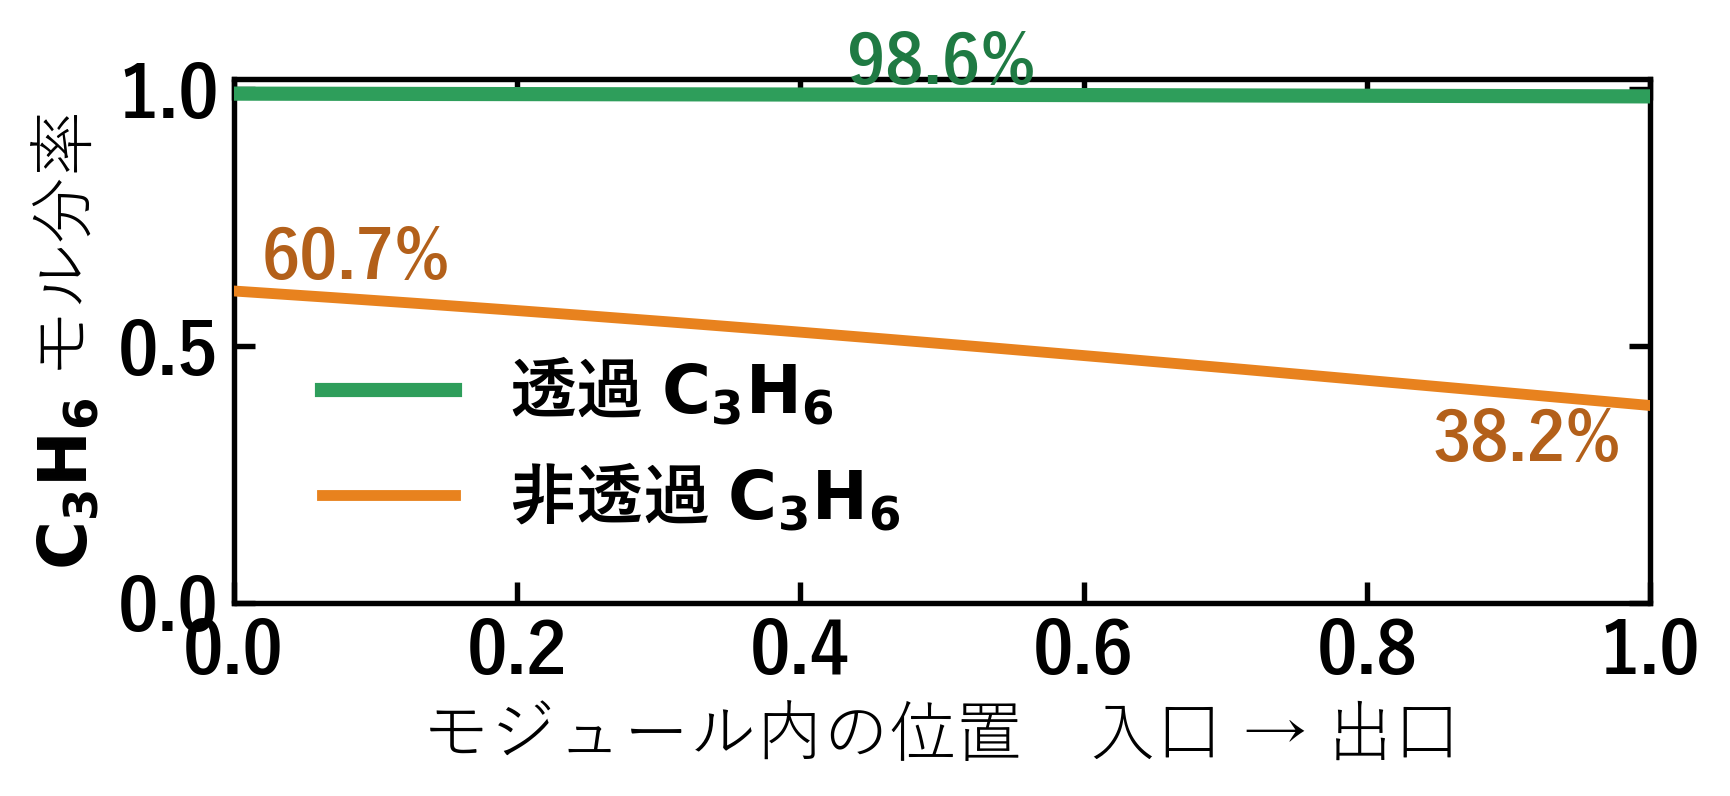
\includegraphics[width=\linewidth]{membrane_profile}\par
      \vspace{-0.82em}
      {\scriptsize モジュール内での $\mathrm{C_3H_6}$ 組成の変化}
    \end{column}
  \end{columns}

  \vspace{0.75em}

  % ===== 下段：設計変数表（左）／膜の選定 枠囲み（右）==========
  \begin{columns}[T,onlytextwidth]
    \begin{column}{0.37\textwidth}
      {\scriptsize\bfseries\color{HeaderBlue} 設計変数と性能}\par
      \vspace{0.12em}
      {\scriptsize\setlength{\tabcolsep}{5pt}\renewcommand{\arraystretch}{0.95}%
       \begin{tabular}{@{}l r@{}}
         \toprule
         供給圧 $P_H$ & $8.4$ bar \\
         膜面積 $A_{\mathrm{mem}}$ & $1.28\times10^{5}$ m$^2$ \\
         \midrule
         選択性 $\alpha$ & $90$ \\
         透過度 $Q_A$ & $40$ GPU \\
         透過圧 $P_L$ & $1$ atm \\
         \midrule
         モジュール数 & $256$ 本 \\
         ステージカット & $37$ \% \\
         透過純度 $\mathrm{C_3H_6}$ & $98.6$ mol\% \\
         \bottomrule
       \end{tabular}}\par
      \vspace{0.12em}
      {\tiny\color{black!55} 上2行が最適化変数\par
       \vspace{0.10em}
       GPU：気体透過率の単位\par
       \smash{$1\,\mathrm{GPU}=3.35\times10^{-10}\ \mathrm{mol\,m^{-2}s^{-1}Pa^{-1}}$}\par
       \vspace{0.6em}
       {\color{black!50} 出典　Hua et al., ACS AMI, 16, 15273, 2024}}
    \end{column}

    \begin{column}{0.63\textwidth}
      {\setlength{\fboxsep}{6pt}\setlength{\fboxrule}{1.2pt}%
       \fcolorbox{SepGreen!55!black}{SepGreen!6}{%
        \begin{minipage}[t][4.0cm]{0.93\linewidth}
         {\scriptsize\bfseries\color{SepGreen!40!black} 膜の選定　ZIF-8 を高分子に分散した混合マトリックス膜}
         \vfill
         {\scriptsize\setlength{\tabcolsep}{4pt}\renewcommand{\arraystretch}{1.1}%
          \begin{tabular}{@{}l c c l@{}}
            \toprule
            膜種 & $\alpha$ & 透過 GPU & 特徴 \\
            \midrule
            多結晶 ZIF-8 & $\sim\!300$ & $52$ & 大面積化・高コスト \\
            高分子膜 & 低 & --- & 可塑化・低性能 \\
            {\bfseries\color{SepGreen!40!black} 採用 混合膜} & {\bfseries 90} & {\bfseries 40} & 量産可・高選択 \\
            \bottomrule
          \end{tabular}}
         \vfill
         {\scriptsize\raggedright 高選択の鍵\par \textbf{小さい非晶質 ZIF-8}・添加剤併用の in-situ 形成で量産\par}
         \vfill
         {\scriptsize\raggedright {\color{SpRed}\textbf{!}}\ 実験室レベル　大面積・連続化で低下＝採用値は楽観側\par}
         \vfill
         {\scriptsize\raggedright 実機の劣化要因：可塑化・競争吸着・濃度分極 等\par}
        \end{minipage}}}
    \end{column}
  \end{columns}

\end{frame}


\section{PSA}
% =====================================================================
%  13  水素分離 — PSA（2段：上=概念図/吸着等温線、下=設計変数表/方式選定）
%  source_memo: 08章＋psa_system.py＋top1_trial201.txt[PSA]。活性炭・多成分Langmuir(Choi2003)
%   ＋LDF・1D PDE。H2非吸着で全量製品、CH4/C2H4/C2H6を吸着。破過基準0.1%。
%   最適化変数: 塔径D4.49m・層高L24.8m・脱着目標β0.254。導出 t_abs742/t_des113s・2基。
%   H2回収~84%・H2純度>99.9%・CH4捕捉100%。入1486(H2 60%)→H2製品746＋オフガス740 kmol/h。
%  方針：図で一目＋口頭。H2=緑、吸着成分=暖色。丸括弧禁止。余白を作らず最下部まで。
% =====================================================================
\definecolor{SepGreen}{HTML}{2E9E5B}
\definecolor{DipeOrange}{HTML}{E8821E}
\begin{frame}[t]

  \vspace{0.1em}

  % ===== 上段：PSA概念図（左）／吸着等温線（右）=================
  \begin{columns}[T,onlytextwidth]
    \begin{column}{0.46\textwidth}
      \raggedright
      {\footnotesize\bfseries\color{HeaderBlue} PSA　圧力スイング吸着}\par
      \vspace{0.3em}
      \centering
      \resizebox{\linewidth}{!}{%
      \begin{tikzpicture}[
        x=1cm, y=1cm, >=Stealth,
        bed/.style={draw, line width=1pt, minimum width=1.4cm, minimum height=2.1cm,
                    align=center, font=\Large\bfseries, rounded corners=2pt},
        io/.style={align=center, font=\Large},
        a/.style={-{Stealth[length=2.8mm]}, line width=1.4pt},
      ]
        \node[bed, draw=HeaderBlue, fill=HiBlue!45, text=HeaderBlue] (A) at (0,0) {吸着\\高圧};
        \node[bed, draw=black!45, fill=black!8, text=black!55] (B) at (2.9,0) {脱着\\低圧};
        % 供給（左→A）
        \node[io, anchor=east] (feed) at (-1.55,0) {供給 $\mathrm{H_2}$ リッチ\\{\normalsize $1486$ kmol/h ・$60$\%}};
        \draw[a, HeaderBlue] (feed.east) -- (A.west);
        % H2 製品（A→上）
        \node[io, anchor=south, text=SepGreen!45!black] (h2) at (0,1.5) {$\mathrm{H_2}$ 製品 $>99.9$\%\\{\normalsize $746$ kmol/h}};
        \draw[a, SepGreen!70!black] (A.north) -- (h2.south);
        % オフガス（B→下）
        \node[io, anchor=north, text=DipeOrange!75!black] (off) at (2.9,-1.45) {オフガス → 燃料\\{\normalsize $740$ kmol/h}};
        \draw[a, DipeOrange!80!black] (B.south) -- (off.north);
        % スイング
        \draw[{Stealth[length=2mm]}-{Stealth[length=2mm]}, line width=0.9pt, black!55]
              (A.east) -- node[above, font=\normalsize, text=black!60]{スイング}(B.west);
      \end{tikzpicture}}
    \end{column}

    \begin{column}{0.54\textwidth}
      \centering
      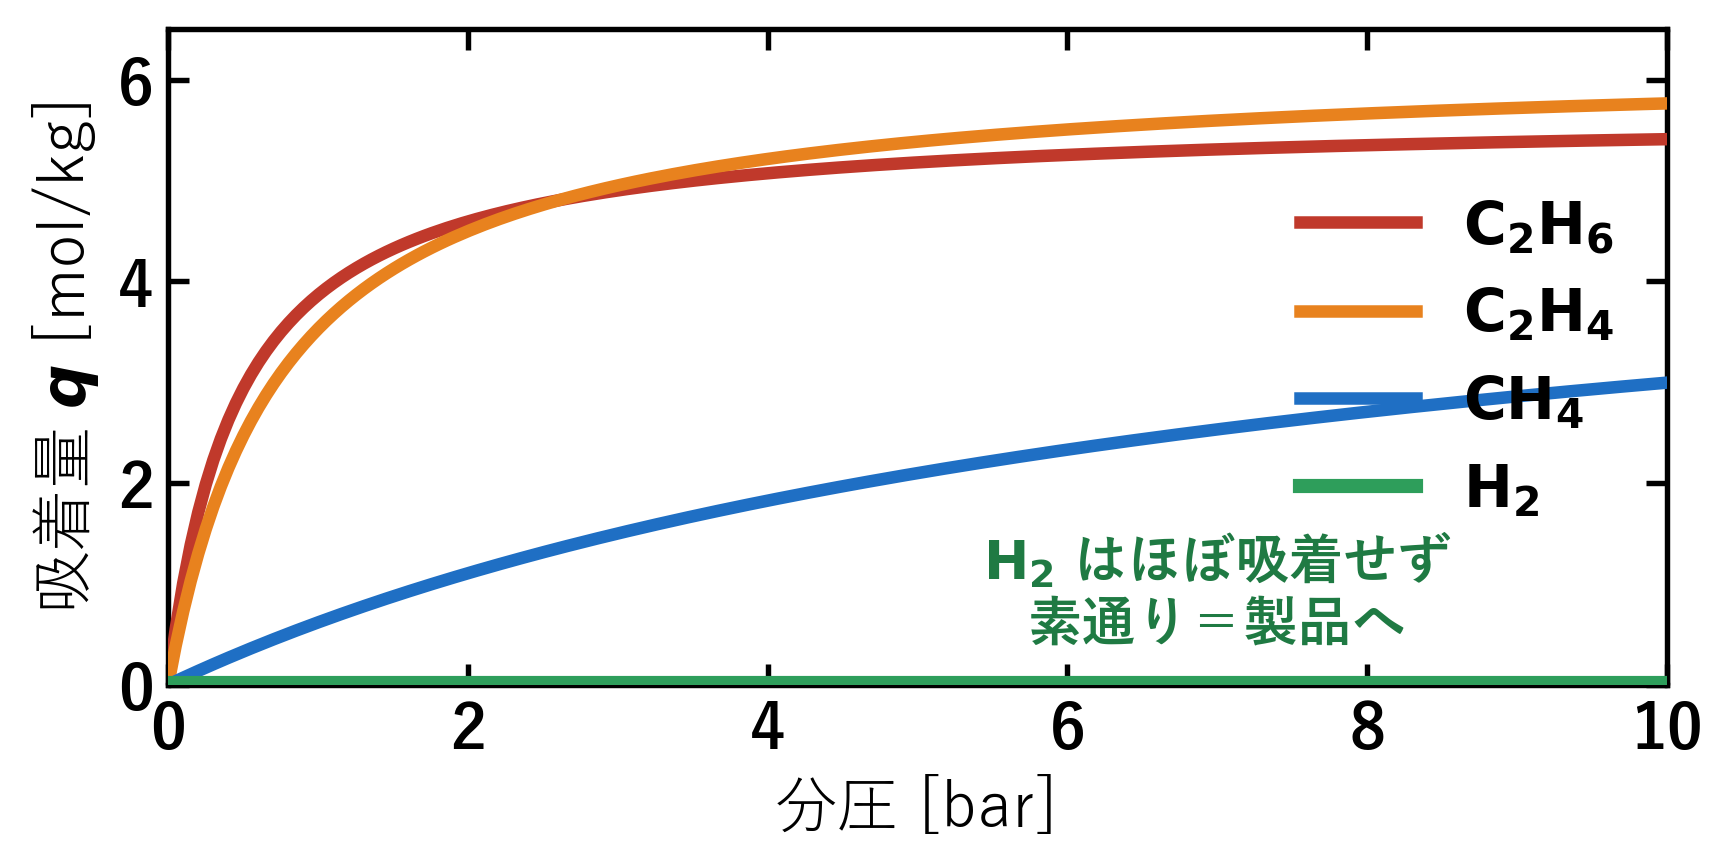
\includegraphics[width=\linewidth]{psa_isotherm}\par
      \vspace{-0.82em}
      {\scriptsize 活性炭の吸着等温線　$25\,^\circ$C}\par
      \vspace{0.12em}
      {\tiny\color{black!55} 出典：B.-U.\ Choi \textit{et al.}, J.\ Chem.\ Eng.\ Data, \textbf{48}(3), 603--607 (2003)}
    \end{column}
  \end{columns}

  \vspace{0.7em}

  % ===== 下段：設計変数表（左）／方式の選定 枠囲み（右）=========
  \begin{columns}[T,onlytextwidth]
    \begin{column}{0.37\textwidth}
      {\scriptsize\bfseries\color{HeaderBlue} 設計変数と諸元}\par
      \vspace{0.12em}
      {\scriptsize\setlength{\tabcolsep}{5pt}\renewcommand{\arraystretch}{1.02}%
       \begin{tabular}{@{}l r@{}}
         \toprule
         塔径 $D$ & $4.49$ m \\
         層高 $L$ & $24.8$ m \\
         脱着目標 $\beta$ & $0.254$ \\
         \midrule
         吸着材 & 活性炭 \\
         塔数 & $2$ 基 \\
         吸着／脱着時間 & $742$／$113$ s \\
         \midrule
         $\mathrm{H_2}$ 純度 & $99.9$\% 超 \\
         $\mathrm{H_2}$ 回収率 & 約 $84$\% \\
         $\mathrm{CH_4}$ 捕捉 & $100$\% \\
         \bottomrule
       \end{tabular}}\par
      \vspace{0.12em}
      {\tiny\color{black!55} 上3行が最適化変数}
    \end{column}

    \begin{column}{0.63\textwidth}
      {\setlength{\fboxsep}{6pt}\setlength{\fboxrule}{1.2pt}%
       \fcolorbox{HeaderBlue!70!black}{HiBlue!12}{%
        \begin{minipage}[t][4.13cm]{0.93\linewidth}
         {\scriptsize\bfseries\color{HeaderBlue} 方式の選定　PSA 圧力スイング吸着}
         \vfill
         {\scriptsize\setlength{\tabcolsep}{4pt}\renewcommand{\arraystretch}{1.1}%
          \begin{tabular}{@{}l c l@{}}
            \toprule
            方式 & $\mathrm{H_2}$ 純度 & 課題 \\
            \midrule
            深冷分離 & 高 & $-170\,^\circ$C 級・高コスト \\
            膜 & 中 & 高純度に多段が必要 \\
            {\bfseries\color{HeaderBlue} 採用 PSA} & {\bfseries $>99.9$\%} & 工業実績・連続 2 基 \\
            \bottomrule
          \end{tabular}}
         \vfill
         {\scriptsize\raggedright 吸着材＝\textbf{活性炭}：$\mathrm{H_2}$ 非吸着・$\mathrm{CH_4}/\mathrm{C_2}$ を選択吸着\par}
         \vfill
         {\scriptsize\raggedright 価値化：$\mathrm{H_2}$ は製品販売・\textbf{オフガスは予熱炉の燃料}\par}
        \end{minipage}}}
    \end{column}
  \end{columns}

\end{frame}


\section{全体最適化}
% =====================================================================
%  14  全体最適化 — 左=手法／評価関数(TAC・CAPEX・OPEX の定義と分類)／制約、
%   右=設計変数22の探索範囲＋最適化で決定した値(赤)。F_freshは従属変数のため非掲載。
%  source_memo: 評価関数・CAPEX/OPEX 定義=03_economic_indicators.tex（TAC=CAPEX/n+OPEX, n=8、
%   OPEX=0.180 C_TM+2.73 C_OL+1.23(C_UT+C_WT+C_RM)）、探索範囲=Z:\pdh_simulator\main.py SEARCH_SPACE、
%   決定値=02_process_overview.tex Table 2.3 / best.json trial #201（スライド3と一致）、
%   制約=Z:\pdh_simulator\flowsheet\specs.py＋units\reactors\catofin.py。
%  方針：帯と本文を重ねない（上 vspace は小さな正）。余白を先に使い、足りない分だけ縮小。
%        評価関数を主役に TAC/CAPEX/OPEX の定義・分類を詳述。決定値は赤＝最適化の出力。丸括弧禁止。
% =====================================================================
\definecolor{SpGreen}{HTML}{1FB24D}   % 製品目標スペック強調用の明るい緑
\begin{frame}[t]

  \vspace*{0.2ex}
  \begin{columns}[T,onlytextwidth]
    % ===== 左：最適化手法・評価関数(TAC/CAPEX/OPEX 詳述)・制約条件 ====
    \begin{column}{0.53\textwidth}
      \fbox{\scriptsize 最適化手法}\;{\footnotesize\bfseries ベイズ最適化(TPE)}\par

      \vspace{0.34em}
      \fbox{\scriptsize 評価関数}\;{\footnotesize 年間総費用 {\color{SpRed}\bfseries TAC} を最小化}\par
      \vspace{0.2em}
      {\normalsize\boldmath$ {\color{SpRed}\mathrm{TAC}}=\mathrm{CAPEX}/n+\mathrm{OPEX} $\unboldmath}\par

      \vspace{0.46em}
      {\raggedright
       {\footnotesize\bfseries CAPEX}\par
       {\scriptsize\linespread{1.05}\selectfont 資本的支出　建設の初期投資\par
        \hspace{0.9em}直接費：機器費・据付・配管・計装・土木\par
        \hspace{0.9em}間接費：設計・予備費・エンジニアリング\par}
       \vspace{0.38em}
       {\footnotesize\bfseries OPEX}\par
       {\scriptsize\linespread{1.05}\selectfont 事業運営費　年間の運転費\par
        \hspace{0.9em}変動費：原料費・用役費・廃棄物処理費\par
        \hspace{0.9em}固定費：労務費・保全費・一般経費\par
        \vspace{0.95em}
        $n$：法定耐用 $8$ 年\par}
      }

      \vspace{0.46em}
      \fbox{\scriptsize 制約条件}\par
      \vspace{0.18em}
      {\scriptsize\linespread{1.0}\selectfont
       \begin{tabular}{@{}p{0.47\linewidth}@{\hspace{0.3em}}|@{\hspace{0.3em}}p{0.50\linewidth}@{}}
         \raggedright
         {\color{SpGreen}・C3H6 純度 $\ge 99.5$ wt\%}\par
         ・H2 純度 $\ge 99.9$ mol\%\par
         {\color{SpGreen}・生産量 $\ge 400$ kt/年}\par
         ・反応器 床$\Delta P\le 5$\%\par
         ・反応器 総$\Delta P\le 10$\%\par
         ・空塔速度 $\ge 0.15$ m/s
         &
         \raggedright
         ・触媒体積 $\le 200\ \mathrm{m^3}$／基\par
         ・PSA 床圧損 $\le 0.3$ bar\par
         ・脱エタン塔頂が凝縮可\par
         ・膜供給圧 $>$ フィード圧\par
         ・リサイクル収支整合
       \end{tabular}}
    \end{column}

    \begin{column}{0.01\textwidth}\end{column}   % 中央の余白

    % ===== 右：設計変数22の探索範囲＋決定値(赤)。ユニットごとに枠を分割 ======
    \begin{column}{0.46\textwidth}
      \setlength{\fboxsep}{1.5pt}\setlength{\fboxrule}{0.8pt}%
      \fcolorbox{HeaderBlue}{white}{\makebox[\dimexpr\linewidth-2\fboxsep-2\fboxrule\relax][l]{%
        \scriptsize\renewcommand{\arraystretch}{0.82}%
        \begin{tabular}{@{}l@{\hspace{0.5em}}l@{\hspace{0.5em}}l@{\hspace{0.6em}}r@{\hspace{0.35em}}l@{}}
          入口温度     & $T_{\mathrm{in}}$  & $930$–$940$   & {\color{SpRed}$935.2$} & K \\
          サイクル時間 & $t_{\mathrm{cyc}}$ & $12$–$25$     & {\color{SpRed}$14.0$}  & min \\
          反応器内径   & $D$                & $9$–$12$      & {\color{SpRed}$10.76$} & m \\
          浅床厚       & $L_{\mathrm{bed}}$ & $0.3$–$3.0$   & {\color{SpRed}$1.58$}  & m \\
          並列基数     & $N_{\mathrm{on}}$  & $6$–$8$       & {\color{SpRed}$7$}     & --- \\
          触媒粒径     & $d_p$              & $4$–$6$       & {\color{SpRed}$5.84$}  & mm \\
        \end{tabular}}}\par\vspace{0.6pt}
      \fcolorbox{HeaderBlue}{white}{\makebox[\dimexpr\linewidth-2\fboxsep-2\fboxrule\relax][l]{%
        \scriptsize\renewcommand{\arraystretch}{0.82}%
        \begin{tabular}{@{}l@{\hspace{0.5em}}l@{\hspace{0.5em}}l@{\hspace{0.6em}}r@{\hspace{0.35em}}l@{}}
          PSA 塔径     & $D_{\mathrm{P}}$   & $2.9$–$5.0$   & {\color{SpRed}$4.49$}  & m \\
          PSA 層高     & $L_{\mathrm{P}}$   & $22$–$30$     & {\color{SpRed}$24.8$}  & m \\
          脱着基準     & $\beta$            & $0.22$–$0.40$ & {\color{SpRed}$0.254$} & --- \\
        \end{tabular}}}\par\vspace{0.6pt}
      \fcolorbox{HeaderBlue}{white}{\makebox[\dimexpr\linewidth-2\fboxsep-2\fboxrule\relax][l]{%
        \scriptsize\renewcommand{\arraystretch}{0.82}%
        \begin{tabular}{@{}l@{\hspace{0.5em}}l@{\hspace{0.5em}}l@{\hspace{0.6em}}r@{\hspace{0.35em}}l@{}}
          膜供給圧     & $P_H$              & $7.5$–$9.5$   & {\color{SpRed}$8.44$}  & bar \\
          膜面積       & $A_{\mathrm{mem}}$ & $0.5$–$3$     & {\color{SpRed}$1.28$}  & $\times10^{5}\,\mathrm{m^2}$ \\
        \end{tabular}}}\par\vspace{0.6pt}
      % 原料流量 F_fresh は最適化変数ではなく従属変数（製品スペック固定下で物質収支から決定、
      % 決定値 1494.6 kmol/h）のため本表から除外（22 変数）。
      \fcolorbox{HeaderBlue}{white}{\makebox[\dimexpr\linewidth-2\fboxsep-2\fboxrule\relax][l]{%
        \scriptsize\renewcommand{\arraystretch}{0.82}%
        \begin{tabular}{@{}l@{\hspace{0.5em}}l@{\hspace{0.5em}}l@{\hspace{0.6em}}r@{\hspace{0.35em}}l@{}}
          塔圧力       & $P_1$ & $16$–$20$    & {\color{SpRed}$19.5$} & bar \\
                       & $P_2$ & $7.7$–$8.2$  & {\color{SpRed}$7.88$} & bar \\
                       & $P_3$ & $16$–$19$    & {\color{SpRed}$16.8$} & bar \\
          塔段数       & $N_1$ & $30$–$60$    & {\color{SpRed}$36$}   & --- \\
                       & $N_2$ & $60$–$80$    & {\color{SpRed}$61$}   & --- \\
                       & $N_3$ & $115$–$160$  & {\color{SpRed}$117$}  & --- \\
          フィード段   & $N_{f1}$ & $22$–$28$ & {\color{SpRed}$28$}   & --- \\
          フィード比   & $f_2$ & $0.40$–$0.60$ & {\color{SpRed}$0.51$} & --- \\
                       & $f_3$ & $0.60$–$0.90$ & {\color{SpRed}$0.82$} & --- \\
          組成分率     & $\phi_1$ & $0.90$–$0.999$ & {\color{SpRed}$0.995$} & --- \\
          還流比       & $R_2$ & $10$–$15$    & {\color{SpRed}$11.8$} & --- \\
        \end{tabular}}}\par
      \vspace{1pt}
      {\tiny {\color{SpRed}\bfseries 赤：決定値}・$1$脱ブタン $2$脱エタン $3$C3塔}
    \end{column}
  \end{columns}

\end{frame}


\section{最適化変数の選定}
% =====================================================================
%  15  最適化変数の選定 — 「変数の最適値は互いに依存＝部分最適化できない」を
%   工程をまたぐ4つの変数ペアの TAC 等高線(全点フローシート HYSYS, trial#201 背景)で示す。
%   どのペアでも最小 TAC の谷が斜め＝2変数の最適値が互いに依存 → 全 23 変数を同時最適化。
%  source_memo: figures/make_interaction_panels.py(+ run_interaction_grid.py /
%   run_interaction_xsub.py が p1..p4 を全フローシート評価)。★＝採用設計。
% =====================================================================
\begin{frame}[t]

  \vspace*{2.0ex}
  {\bfseries\normalsize 最適値が相互依存　$\to$　全 23 変数を同時最適化}\par

  \vspace{0.6ex}
  \centering
  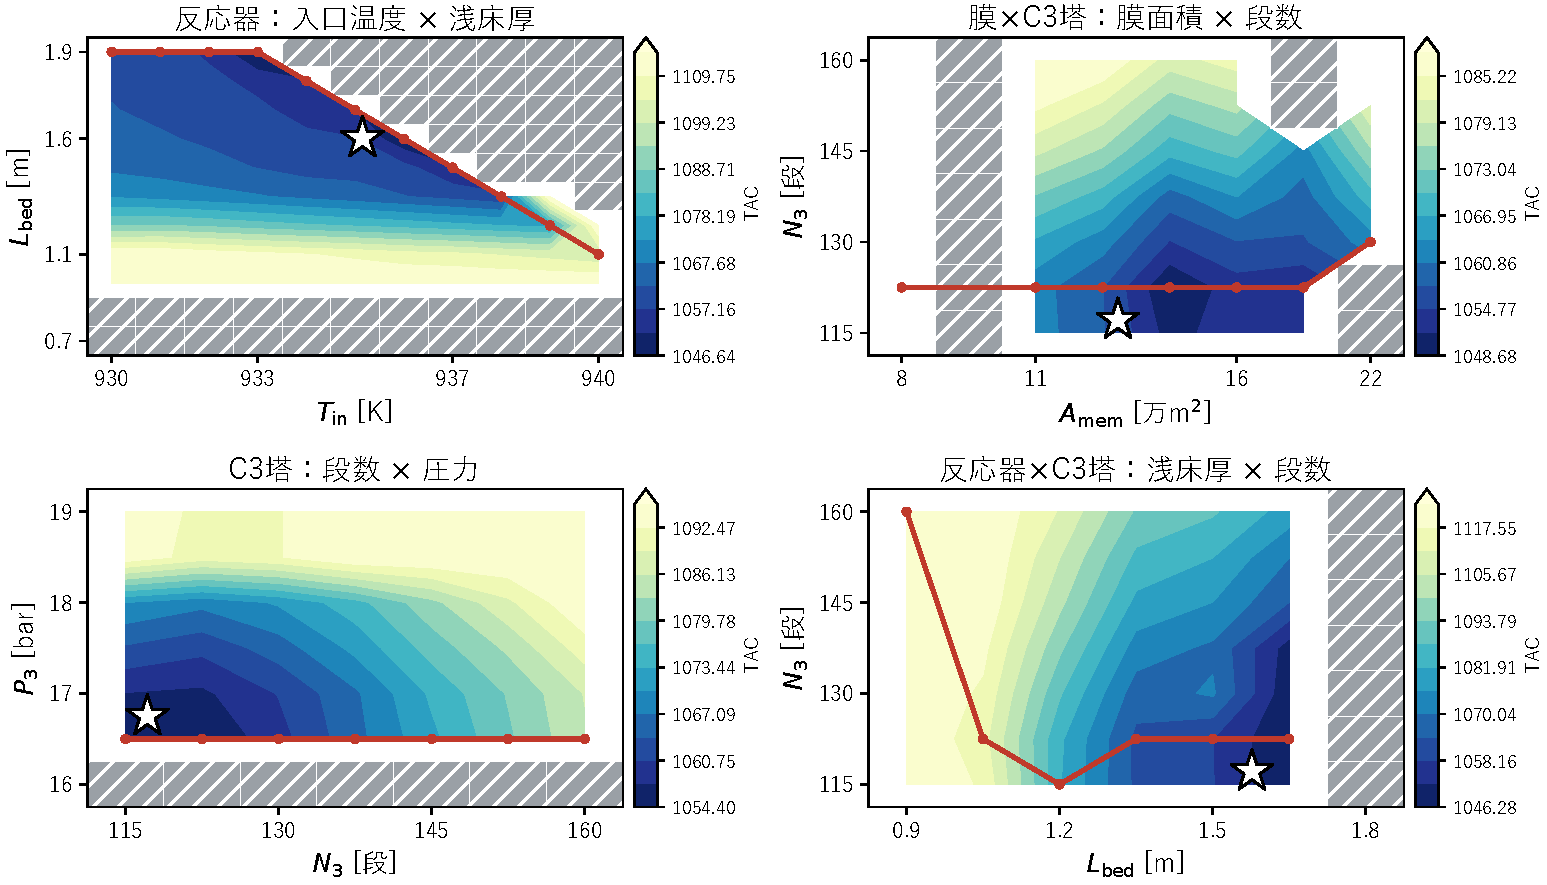
\includegraphics[width=0.95\linewidth]{fig_interaction_panels}\par
  \vspace{0.2ex}
  {\scriptsize 各ペアの TAC 等高線（☆：採用設計・灰：制約違反・{\color{SpRed}赤線}：各列で TAC 最小の点＝谷底）}\par
  \vspace{0.25em}
  {\scriptsize どのユニットでも 2 変数の最適な組合せは互いに依存し独立に決められない}

\end{frame}


\section{経済分析}
% =====================================================================
%  16  経済分析 — 費用/収益・OPEX/CAPEX 内訳（上段）と世界 PDH 立地（下段）
%  source_memo: 10_optimization.tex §経済性・12_analysis_discussion.tex §採算性/立地。
%   図 figures/make_econ_breakdown_slide.py（棒＋OPEX/CAPEX ドーナツ, OPEX は HI 後）と
%      figures/make_econ_map_slide.py（米州｜欧中亜の 2 パネル）。
%   いずれも graph/make_charts.py・make_map.py と同一データをスライド用に変換。
%  方針：見出し文は置かず図で語らせる。図は \paperwidth で左右フルブリード、
%   上は帯直下・下は最下部まで使い、余白を最小化する。丸括弧禁止。
% =====================================================================
\begin{frame}[t]

  \vspace*{6mm}   % 帯とタイトルの重なり回避：内容を明示的に下げる（[t] では \fill が効かないため）
  \centering
  \makebox[\linewidth]{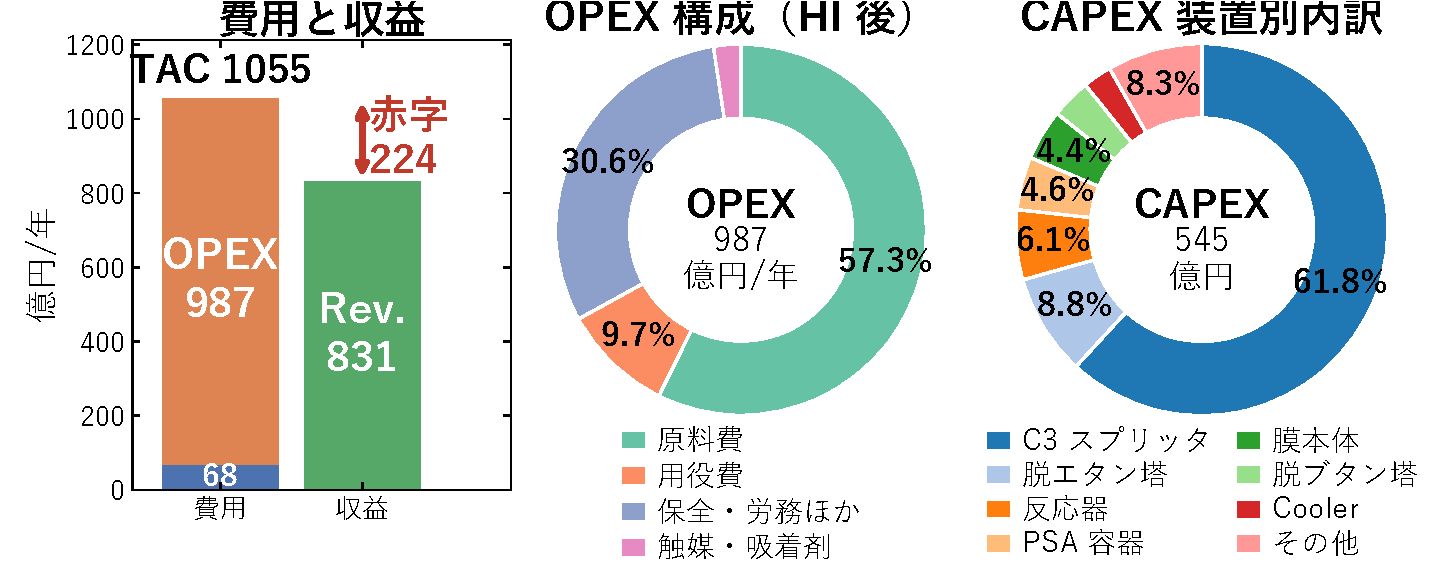
\includegraphics[width=\paperwidth]{econ_breakdown_slide}}\par

  \vspace{0.1em}
  \makebox[\linewidth]{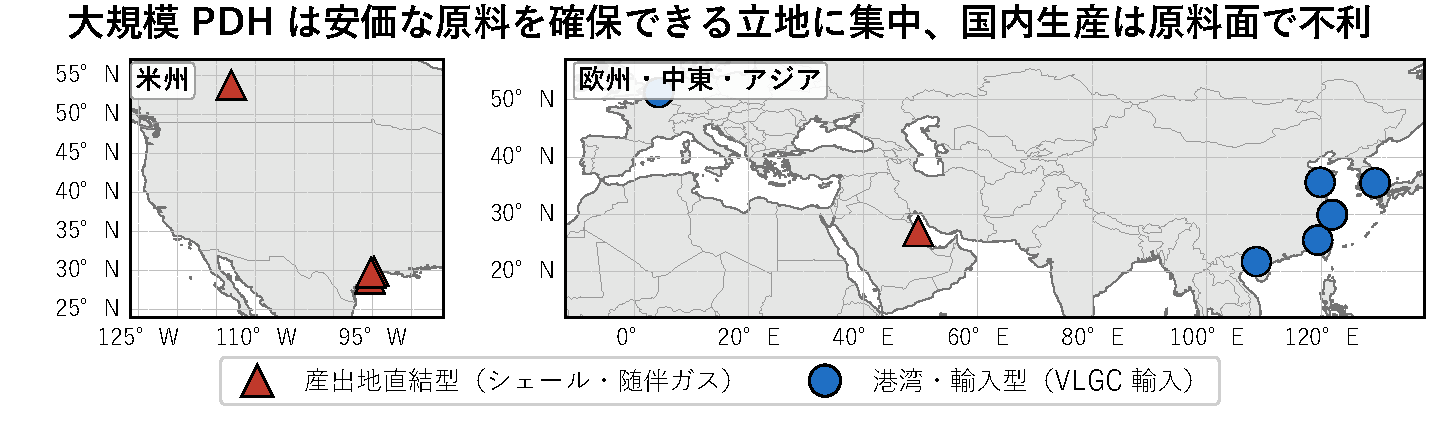
\includegraphics[width=\paperwidth]{econ_map_slide}}

\end{frame}


\section{結言}
% =====================================================================
%  17  結言 — 上=損益分岐の短い解説／損益分岐図、下=結言＋改善案8項目
%  source_memo: 全章。損益分岐図=breakeven_slide.png（最良設計点固定でLPG単価を振り年間利益、
%   分岐64.4円/kg・現行95円/kgで赤字224億円/年）。結言文=指定どおり。
%  方針：図で一目＋口頭。色は赤字数値のみ。丸括弧禁止。余白を作らず最下部まで。
% =====================================================================
\begin{frame}[t]

  \vspace{0.15em}

  % ===== 上段：短い解説（左）／損益分岐図（右）=================
  \begin{columns}[T,onlytextwidth]
    \begin{column}{0.50\textwidth}
      \vspace{0.3em}
      {\small\raggedright
        最良設計点を固定し、\textbf{LPG 原料単価を振って年間利益}を評価。\par
        \vspace{0.45em}
        損益分岐点は \textbf{LPG $64.4$ 円/kg}。現行 $95$ 円/kg では {\color{SpRed}\textbf{赤字 $224$ 億円/年}}。\par
        \vspace{0.45em}
        $\to$ \textbf{安価な原料が得られる立地なら黒字化}。\par}
    \end{column}
    \begin{column}{0.50\textwidth}
      \centering
      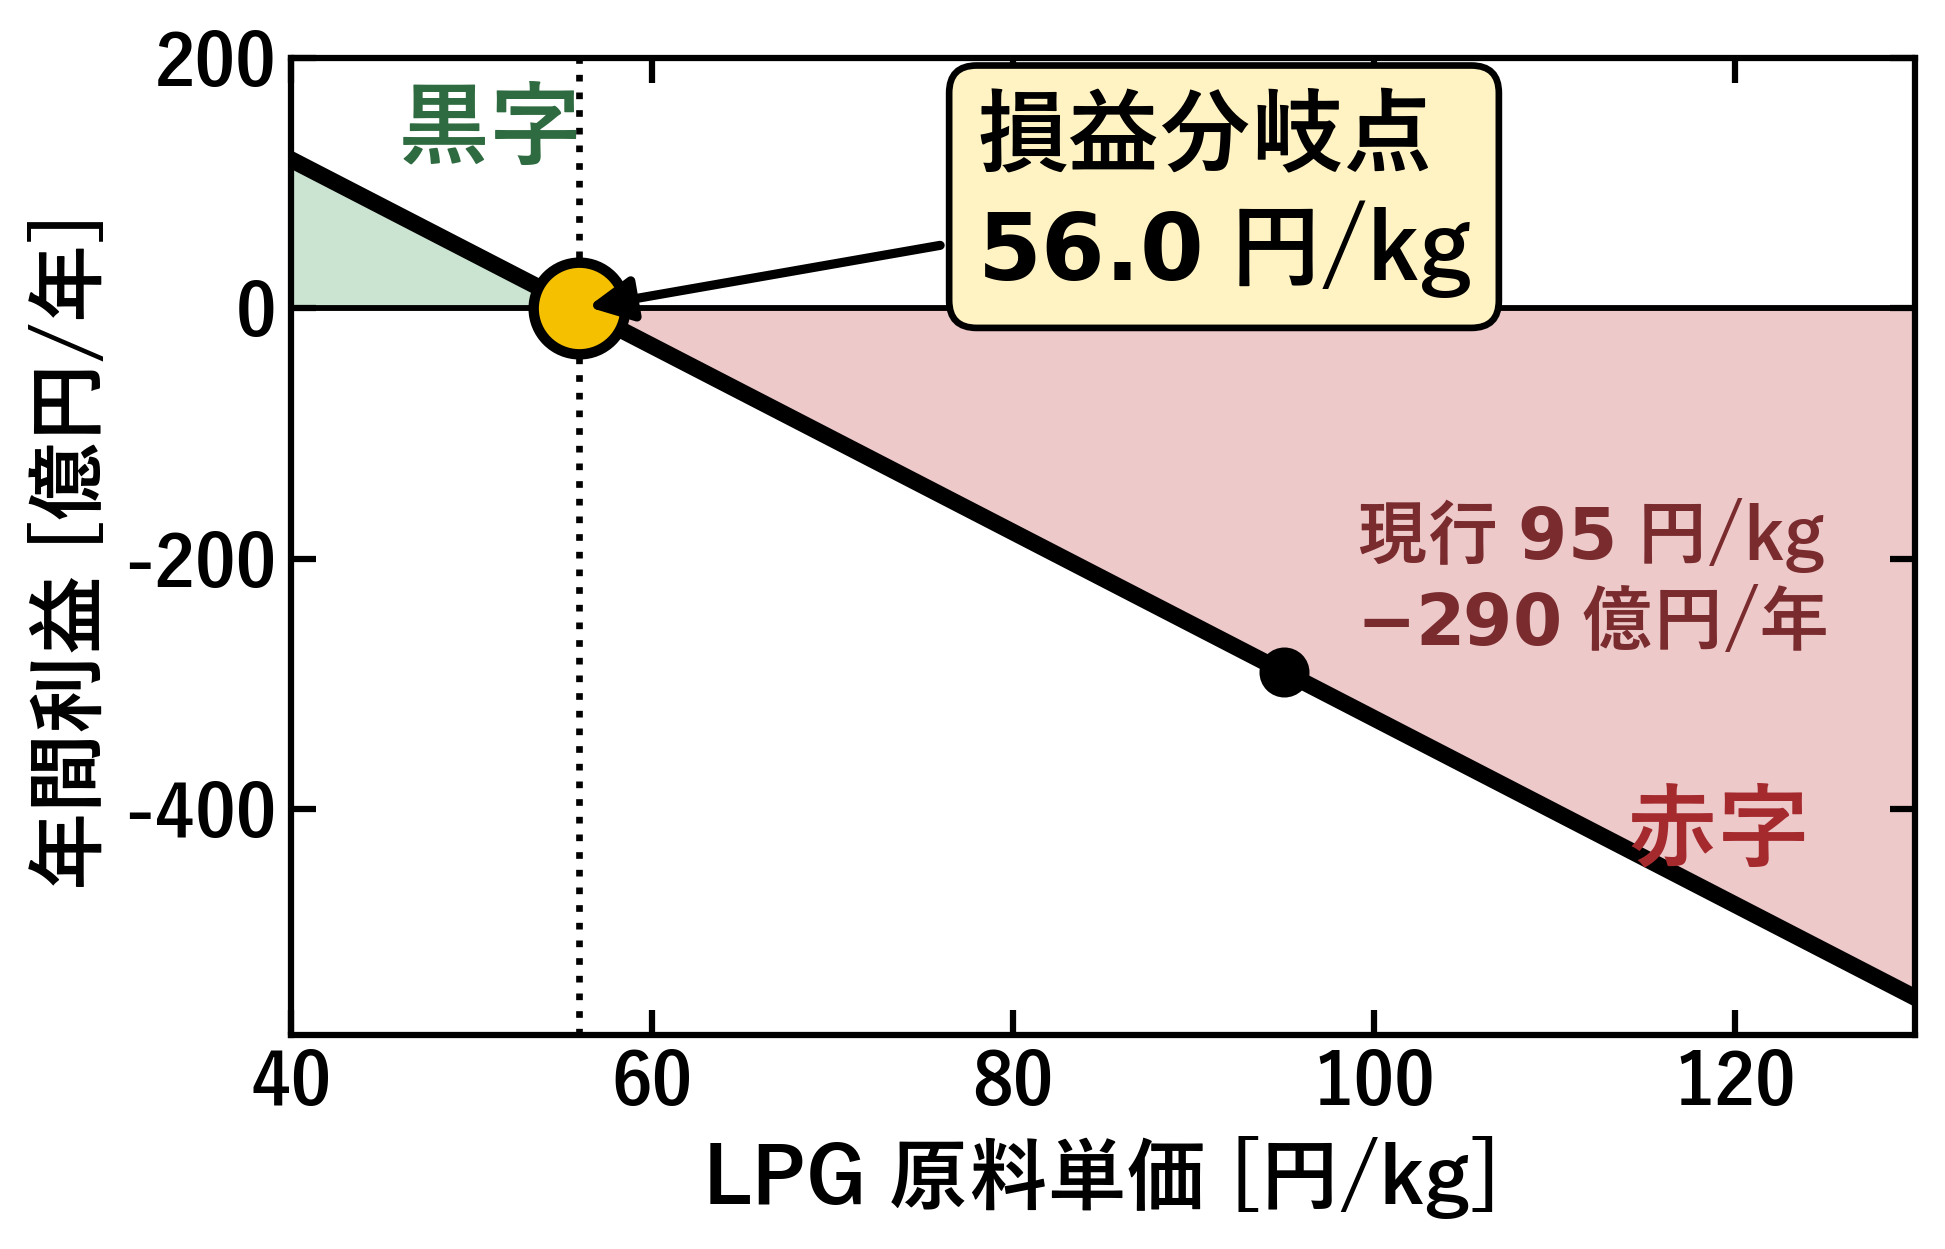
\includegraphics[width=\linewidth]{breakeven_slide}
    \end{column}
  \end{columns}

  \vspace{0.6em}

  % ===== 中段：結言（枠）=======================================
  {\setlength{\fboxsep}{6pt}\setlength{\fboxrule}{1.2pt}%
   \fcolorbox{HeaderBlue}{HiBlue!10}{%
    \begin{minipage}{\dimexpr\linewidth-16pt}
     {\footnotesize\bfseries\color{HeaderBlue} 結言}\quad
     {\small LPG から PDH でプロピレン {\boldmath$402$} kt/年・{\boldmath$99.5$} wt\% を製造する全プロセスを設計し、\textbf{全 $23$ 変数の同時最適化で TAC を最小化}した。}
    \end{minipage}}}

  \vspace{0.55em}

  % ===== 下段：改善案 8項目（小文字・行間詰め・2列）===========
  {\footnotesize\bfseries\color{HeaderBlue} 改善案}\par
  \vspace{0.2em}
  {\scriptsize\setlength{\parskip}{0.1em}
   \begin{columns}[T,onlytextwidth]
    \begin{column}{0.5\textwidth}
      \raggedright
      $\bullet$ \textbf{触媒の選定}：高選択・高活性触媒の探索\par
      $\bullet$ \textbf{触媒形状の改良}：中心にダミーを入れ実効粒径を拡大 $\to$ 圧損低減\par
      $\bullet$ \textbf{膜の経時劣化}をモデル化し現実性能で再評価\par
      $\bullet$ \textbf{熱交換器ネットワーク HEN の本格合成}\par
      $\bullet$ 熱交換網の\textbf{最小接近温度差 $\Delta T_{\min}$ を最適化変数に追加}\par
    \end{column}
    \begin{column}{0.5\textwidth}
      \raggedright
      $\bullet$ \textbf{反応速度論・選択率モデル}の高精度化\par
      $\bullet$ \textbf{非定常・動特性／制御性}の検討\par
      $\bullet$ \textbf{多目的最適化}：TAC に $\mathrm{CO_2}$・安全性を併せ評価\par
      $\bullet$ \textbf{安価 LPG の調達・立地}最適化と不確実性下のロバスト設計\par
    \end{column}
   \end{columns}}

\end{frame}


% ===== 参考・注釈／付録（ページ番号は 18/17… と本線17枚を超える）=====
\section{参考・注釈}
% =====================================================================
%  18  参考・注釈 — 中央2分割：左=使用ツール・手法／右=参考文献・出典
%  方針：丸括弧禁止・体言止め・装飾なし（青色/枠なし、黒文字のみ）・
%        小さめフォント＋自然な位置で手動改行し下手な改行を排除・
%        ツール名/文献名を太字・縦は中央寄せで余白を均す。
%  ※ 引用は原則「使った箇所の文中／文章の直下」に置く。本スライドは他に
%    載せどころのない横断的な出典（物性・コスト・課題データ）のみを置く。
%  付録扱い：ページ番号は 18/17 となり本線17枚を超えることで本線と区別。
% =====================================================================
\begin{frame}[t]

  \vfill

  \begin{columns}[T,onlytextwidth]
    % ---- 左：使用ツール・手法 ----
    \begin{column}{0.5\textwidth}
      {\footnotesize\bfseries 使用ツール}\par
      \vspace{0.7em}
      {\scriptsize\raggedright\linespread{1.3}\selectfont
        \textbf{蒸留塔の設計・計算}\par
        Aspen HYSYS\par
        \vspace{0.7em}
        \textbf{反応器・分離・最適化の自作計算}\par
        Python の主要モジュール\par
        ・\textbf{SciPy}：反応器の常微分方程式積分・気液平衡計算\par
        ・\textbf{Optuna}：全 22 変数の最適化、TPE／CMA-ES\par
        ・\textbf{thermo・chemicals}：物性・状態方程式 PR\par
        ・\textbf{scikit-learn}：実現可能領域の判別解析\par
        ・\textbf{NumPy・pandas・Matplotlib}：数値処理・作図\par
      }
    \end{column}
    % ---- 右：参考文献・出典 ----
    \begin{column}{0.5\textwidth}
      {\footnotesize\bfseries 参考文献・出典}\par
      \vspace{0.7em}
      {\scriptsize\raggedright\linespread{1.3}\selectfont
        \textbf{物性値・各ユニットのモデル化}\par
        改訂六版 化学工学便覧、化学工学会\par
        \vspace{0.6em}
        \textbf{設備費・用役費のコスト推算}\par
        長谷部伸治・外輪健一郎\\
        「プロセス設計 No.\,3 建設費と運転費の推算」\par
        \vspace{0.6em}
        \textbf{物価補正の指標 CEPCI}\par
        Chemical Engineering 誌 Plant Cost Index\\
        2026 年 1 月公表値 $840.6$ を使用\par
        \vspace{0.6em}
        \textbf{熱統合・熱交換器ネットワークの最適合成}\par
        長谷部伸治・外輪健一郎\\
        「プロセスシステム工学 No.\,4\\熱交換器ネットワークの最適合成」\par
        \vspace{0.6em}
        \textbf{反応速度式・触媒活性データおよび生産諸条件}\par
        第 17 回プロセスデザイン学生コンテスト要項\par
      }
    \end{column}
  \end{columns}

  \vfill

\end{frame}


\section{付録目次}
% =====================================================================
%  19  付録目次 — 左上にタイトル「付録」、その下に確定済みの付録目次。
%  運用：付録スライドを追加・変更したらこの目次も同時に更新する
%        （番号＝実ページ番号。現在 20〜30 の 11 枚）。
%  表記：ページ番号は 19/17 と本線 17 枚を超えることで付録と区別する。
%  ルール：丸括弧禁止・最小色・[t] フレーム・帯と本文の重なり禁止・
%        負の上 \vspace* 禁止。
% =====================================================================
\begin{frame}[t]

  \vspace*{3.5mm}
  {\bfseries\large 付録}\par
  \vspace{0.9em}

  {\footnotesize\raggedright\linespread{1.45}\selectfont
    20　コスト推算 1\par
    21　コスト推算 2\par
    22　コスト推算 3\par
    23　反応器仮定検証\par
    24　膜分離原理\par
    25　PSA 原理 1\par
    26　PSA 原理 2\par
    27　PSA 検証\par
    28　発熱材\par
    29　TPE\par
  }

\end{frame}


\section{コスト推算 1}
% =====================================================================
%  20  付録 コスト推算 1 — CAPEX 建設費の推算（Bare Module Cost 法）
%  source_memo: 03_economic_indicators.tex §3.2 ＋ src/cost_calculator.py
%   (calc_cp0 / calc_fp / calc_*_capex) ＋ src/cost_parameters.py。
%   長谷部・外輪「プロセス設計 No.3 建設費と運転費の推算」準拠。
%  方針：シミュレータが使う式と定数をそのまま提示。式の各段に役割ラベル。丸括弧禁止。
% =====================================================================
\begin{frame}[t]

  \vspace*{1.2mm}
  {\footnotesize 機器ごとに体積・伝熱面積・動力からコストを積み上げる
   \textbf{Bare Module Cost 法}。炭素鋼・常圧の標準機器費を基準に、圧力・材質・物価で補正する。}\par

  \vspace{0.55em}
  \begin{columns}[T,onlytextwidth]
    % ===== 左：式の連鎖（各段に役割ラベル）=====
    \begin{column}{0.585\textwidth}
      \fbox{\scriptsize\bfseries 1\ \ 基本コスト $C_p^0$}\;{\scriptsize 炭素鋼・常圧の標準機器費}\par
      \vspace{0.2em}
      {\small\boldmath$C_p^0 = 10^{\,K_1 + K_2\log_{10}\!A + K_3(\log_{10}\!A)^2}$\unboldmath}\par
      {\scriptsize $A$：体積・伝熱面積・動力 などの特徴サイズ}\par

      \vspace{0.55em}
      \fbox{\scriptsize\bfseries 2\ \ モジュール係数 $F_{BM}$}\par
      \vspace{0.15em}
      {\scriptsize 圧力・材質で割増、据付配管計装込み}\par
      \vspace{0.2em}
      {\small\boldmath$F_{BM} = B_1 + B_2\,F_p\,F_M$\unboldmath}\par

      \vspace{0.55em}
      \fbox{\scriptsize\bfseries 3\ \ ベアモジュール費 $C_{BM}$}\;{\scriptsize 1 機の据付完了費}\par
      \vspace{0.2em}
      {\small\boldmath$C_{BM} = C_p^0\,F_{BM}$\unboldmath}\par

      \vspace{0.55em}
      \fbox{\scriptsize\bfseries 4\ \ 総建設費 ${\color{SpRed}\mathrm{CAPEX}}=C_{TM}$}\par
      \vspace{0.15em}
      {\scriptsize 全機器合計＋物価・為替・間接費}\par
      \vspace{0.2em}
      {\small\boldmath${\color{SpRed}\mathrm{CAPEX}}=1.18\times\dfrac{\mathrm{CEPCI_{2026}}}{\mathrm{CEPCI_{base}}}\times\sum_{k}C_{BM,k}$\unboldmath}\par
    \end{column}

    \begin{column}{0.015\textwidth}\end{column}

    % ===== 右：基準定数・圧力係数 =====
    \begin{column}{0.40\textwidth}
      {\scriptsize\bfseries\color{HeaderBlue} 基準定数}\par
      \vspace{0.15em}
      {\setlength{\fboxsep}{4pt}\setlength{\fboxrule}{0.8pt}%
       \fcolorbox{HeaderBlue}{white}{%
        \begin{minipage}{\dimexpr\linewidth-2\fboxsep-2\fboxrule\relax}
        {\scriptsize\setlength{\tabcolsep}{3pt}\renewcommand{\arraystretch}{1.12}%
         \begin{tabular}{@{}l r@{}}
           物価指数 基準 & $397$ \;2001 年 \\
           物価指数 現在 & {\color{SpRed}$840.6$} \;2026 年 \\
           為替 & $158.9$ 円/USD \\
           据付・間接費 & $\times 1.18$ \\
           材質係数 $F_M$ & $1.0$ 炭素鋼 \\
           反応器スイング & $K_{\mathrm{sw}}=1.5$ \\
         \end{tabular}}
        \end{minipage}}}\par

      \vspace{0.7em}
      {\scriptsize\bfseries\color{HeaderBlue} 圧力係数 $F_p$　縦型容器}\par
      \vspace{0.2em}
      {\scriptsize $F_p=\dfrac{(P_g+1)\,D}{10.71-0.00756(P_g+1)}+0.5$}\par
      \vspace{0.3em}
      {\scriptsize $P_g$：ゲージ圧 bar、$D$：内径 m\par
       下限 $F_p\ge1$、真空 $P_g\le-0.5$ では $1.25$}\par

      \vspace{0.7em}
      {\scriptsize 推算レベル　Study estimate\par
       推算精度　$-20$ ～ $+30$ \%}\par
    \end{column}
  \end{columns}

\end{frame}


\section{コスト推算 2}
% =====================================================================
%  21  付録 コスト推算 2 — 機器別の係数とサイジング指標
%  source_memo: 03_economic_indicators.tex Table tab:cost_coefficients ＋
%   src/cost_parameters.py（各機器 K1-K3/B1-B2/FBM）＋ src/cost_calculator.py
%   （calc_cp0/calc_he/calc_comp/calc_pump/calc_tray/calc_mem）。
%   長谷部・外輪「プロセス設計 No.3」付録 Table A.1/A.4 準拠。
%  方針：シミュレータが機器ごとに使う係数を 1 表で提示。丸括弧禁止・最小色。
% =====================================================================
\begin{frame}[t]

  \vspace*{1.2mm}
  {\footnotesize 機器タイプごとに下表の係数で $C_p^0$ と $F_{BM}$ を計算する。
   コストは\textbf{サイジング指標}で決まり、機器の規模が大きいほど単位あたりは割安になる。}\par

  \vspace{0.7em}
  \centering
  {\scriptsize\setlength{\tabcolsep}{5pt}\renewcommand{\arraystretch}{1.32}%
   \begin{tabular}{@{}l l c c c c c@{}}
     \toprule
     機器 & サイジング指標 $A$ & $K_1$ & $K_2$ & $K_3$ & $B_1$ & $B_2$ \\
     \midrule
     縦型容器     & 容器体積 $[\mathrm{m^3}]$  & $3.4974$ & $0.4485$  & $0.1074$ & $2.25$ & $1.82$ \\
     熱交換器     & 伝熱面積 $[\mathrm{m^2}]$  & $4.3247$ & $-0.3030$ & $0.1634$ & $1.63$ & $1.66$ \\
     遠心圧縮機   & 流体動力 $[\mathrm{kW}]$   & $2.2897$ & $1.3604$  & $-0.1027$ & \multicolumn{2}{c}{$F_{BM}=2.15$ 固定} \\
     遠心ポンプ   & 流体動力 $[\mathrm{kW}]$   & $3.3892$ & $0.0536$  & $0.1538$ & $1.89$ & $1.35$ \\
     シーブトレイ & トレイ面積 $[\mathrm{m^2}]$ & $2.9949$ & $0.4465$  & $0.3961$ & \multicolumn{2}{c}{$F_{BM}=1.0$} \\
     膜モジュール & 総膜面積 $[\mathrm{m^2}]$  & \multicolumn{5}{c}{Bare Module 適用外 — 単価 $50$ USD/m$^2$ を直接乗算} \\
     \bottomrule
   \end{tabular}}\par

  \vspace{0.9em}

  \begin{columns}[T,onlytextwidth]
    % ===== 左：各機器が何に対応するか =====
    \begin{column}{0.52\textwidth}
      {\scriptsize\bfseries\color{HeaderBlue} 本プロセスでの対応機器}\par
      \vspace{0.25em}
      {\scriptsize\raggedright\linespread{1.25}\selectfont
       縦型容器　反応器・蒸留塔本体・PSA 塔\\
       \hspace{4.5em}{\color{SpRed}反応器は $K_{\mathrm{sw}}=1.5$}\par
       熱交換器　凝縮器・リボイラ・冷却器・気化器\par
       遠心圧縮機　反応器出口 $2$ 段・膜フィード・膜製品\par
       遠心ポンプ　原料 LPG\quad シーブトレイ　全蒸留塔\par}
    \end{column}

    \begin{column}{0.02\textwidth}\end{column}

    % ===== 右：補正係数の式 =====
    \begin{column}{0.46\textwidth}
      {\scriptsize\bfseries\color{HeaderBlue} 段数補正 $F_q$　トレイ $N<20$ で割高}\par
      \vspace{0.2em}
      {\scriptsize $\log_{10}F_q = 0.4771 + 0.08516\,\ell - 0.3473\,\ell^{2}$,\ \ $\ell=\log_{10}\!N$}\par
      \vspace{0.2em}
      {\scriptsize $C_{BM,\mathrm{tray}} = C_p^0\,N\,F_{BM}\,F_q$\quad $N\ge20$ では $F_q=1$}\par

      \vspace{0.55em}
      {\scriptsize\bfseries\color{HeaderBlue} 材質・圧力}\par
      \vspace{0.2em}
      {\scriptsize\raggedright 全機器 炭素鋼 $F_M=1.0$。圧縮機は $F_p=1.0$、
       ポンプは吐出 $P_g>10$ bar で $F_p$ 補正。}\par
    \end{column}
  \end{columns}

\end{frame}


\section{コスト推算 3}
% =====================================================================
%  22  付録 コスト推算 3 — OPEX 運転費の推算と単価・TAC
%  source_memo: 03_economic_indicators.tex §3.3 ＋ flowsheet/economics.py
%   （apply_hasebe_aggregation / _compute_labor_cost / collect_capex_opex）
%   ＋ src/cost_parameters.py（単価）＋ utility_selector.py（用役階層）。
%   長谷部・外輪「プロセス設計 No.3」§3.3/§3.4 準拠。
%  方針：OPEX 経験式と単価をシミュレータの実装どおり提示。丸括弧禁止・最小色。
% =====================================================================
\begin{frame}[t]

  \vspace*{1.2mm}
  {\footnotesize 年間運転費 OPEX は\textbf{長谷部・外輪の経験式}で推算。原料・用役の実費に、
   保全・労務・諸経費を経験係数で上乗せする。}\par

  \vspace{0.5em}
  {\small\boldmath$\mathrm{OPEX}=0.180\,C_{TM}+2.73\,C_{OL}+1.23\,(C_{UT}+C_{WT}+C_{RM})$\unboldmath}\par
  \vspace{0.2em}
  {\scriptsize $C_{TM}$ 建設費 ｜ $C_{OL}$ 労務費 ｜ $C_{UT}$ 用役費 ｜ $C_{WT}$ 廃棄物費 $=0$ ｜ $C_{RM}$ 原料費\\
   {\color{black!60}＋ 触媒・吸着剤・膜の交換費を別建て}}\par

  \vspace{0.7em}
  \begin{columns}[T,onlytextwidth]
    % ===== 左：労務費の式 ＋ 別建て交換費 =====
    \begin{column}{0.50\textwidth}
      {\scriptsize\bfseries\color{HeaderBlue} 労務費 $C_{OL}$　主要機器数から運転員数を決定}\par
      \vspace{0.2em}
      {\scriptsize $N_{OL}=\big\lceil\sqrt{6.29+0.21\,N_{\mathrm{eq}}}\,\big\rceil$\quad $1$ 班の運転員数}\par
      \vspace{0.15em}
      {\scriptsize $4$ 直 $\to$ 総員 $=4\,N_{OL}$、年俸 $600$ 万円/人\par
       $N_{\mathrm{eq}}$：反応器・塔・圧縮機・熱交換器などの数}\par

      \vspace{0.7em}
      {\scriptsize\bfseries\color{HeaderBlue} 別建て交換費　経験式の枠外・$1.23$ 倍なし}\par
      \vspace{0.2em}
      {\scriptsize\setlength{\tabcolsep}{4pt}\renewcommand{\arraystretch}{1.2}%
       \begin{tabular}{@{}l l@{}}
         触媒 $\mathrm{Cr_2O_3}$ & $23$ USD/kg $\div$ 寿命 $2.5$ 年 \\
         PSA 活性炭 & $5$ USD/kg $\div$ $4$ 年 \\
         膜モジュール & 膜本体 CAPEX $\div$ $3$ 年 \\
       \end{tabular}}\par
    \end{column}

    \begin{column}{0.02\textwidth}\end{column}

    % ===== 右：単価一覧 =====
    \begin{column}{0.47\textwidth}
      {\scriptsize\bfseries\color{HeaderBlue} 原料・製品・用役の単価}\par
      \vspace{0.2em}
      {\setlength{\fboxsep}{4pt}\setlength{\fboxrule}{0.8pt}%
       \fcolorbox{HeaderBlue}{white}{%
        \begin{minipage}{\dimexpr\linewidth-2\fboxsep-2\fboxrule\relax}
        {\scriptsize\setlength{\tabcolsep}{3pt}\renewcommand{\arraystretch}{1.18}%
         \begin{tabular}{@{}l r@{}}
           原料 LPG & $95$ 円/kg \\
           製品 $\mathrm{C_3H_6}$ & {\color{SpRed}$150$} 円/kg \\
           製品 $\mathrm{H_2}$ & {\color{SpRed}$400$} 円/kg \\
           \midrule
           電力 & $17$ 円/kWh \\
           蒸気 LP/MP/HP & $1050$/$1120$/$1330$ 円/GJ \\
           燃料 & $1830$ 円/GJ \\
           冷媒 & Carnot 動力で算定 \\
         \end{tabular}}
        \end{minipage}}}\par
      \vspace{0.18em}
      {\tiny\color{black!55} 用役単価は海外 TEA 文献に CEPCI・為替補正。稼働 $8000$ h/年}\par
    \end{column}
  \end{columns}

  \vspace{0.8em}
  % ===== 最下部：TAC のまとめ帯 =====
  {\setlength{\fboxsep}{5pt}%
   \noindent\colorbox{HiBlue}{%
    \begin{minipage}{\dimexpr\linewidth-2\fboxsep\relax}
     \centering\small\boldmath
     {\color{SpRed}\textbf{TAC}}$\ =\ \mathrm{CAPEX}\,/\,8\ \text{年}\ +\ \mathrm{OPEX}$
     \unboldmath{\footnotesize\quad 建設費を $8$ 年で回収した年資本費＋年運転費}
    \end{minipage}}}

\end{frame}


\section{反応器仮定検証}
% =====================================================================
%  23  付録 反応器仮定検証 — 骨格（スライド3と同じく現状は意図的に空白）
%  source_memo 候補: 04_reaction.tex の検証 Table＋tools/_diffusion_dp_sensitivity.py
%   （Weisz-Prater・Mears で η≈1 を確認）＋_probe_catofin_trial201.py
%   （u・ΔP/P・Q_HGM・N_total の実走値）。
%  ルール：丸括弧禁止・最小色・[t] フレーム・帯と本文の重なり禁止。
% =====================================================================
\begin{frame}[t]

  % ↓↓↓ 中身ができたらここに置く ↓↓↓

\end{frame}


\section{膜分離原理}
% =====================================================================
%  24  付録 膜分離原理 — 分子ふるい × 分圧差駆動の溶解拡散・クロスフローモデル
%  source: 07_product_purification.tex §7.2（膜分離モジュール）
%   §7.2.1 材料・性能（ZIF-8 MMM・Q_A=40 GPU・α=90、Hua et al. 2024）
%   §7.2.2 前提（クロスフロー・等温等圧・線形透過則・透過度の組成圧力非依存）
%   §7.2.3 フラックス J=Q·Δp と膜面積方向の物質収支 dF/dA=-J
%   §7.2.4 局所透過組成 y_loc（クロスフロー二次式）／§7.2.5 モジュール本数
%   分子ふるい数値は figures/make_sieving.py（C3H6 4.0Å 透過・C3H8 4.3Å 阻止）。
%  方針：左＝分子ふるい図で原理、右＝モデル式。膜=緑 SepGreen。丸括弧禁止・最小色・
%   [t] フレーム・帯と本文の重なり禁止（見出しは正値 vspace で帯から離す）。
% =====================================================================
\definecolor{SepGreen}{HTML}{2E9E5B}
\definecolor{DipeOrange}{HTML}{E8821E}
\begin{frame}[t]

  \vspace*{2.4mm}   % \large 見出しを帯から離す（負の上 vspace は禁止、正値で下げる）
  {\bfseries\large 膜分離の原理　分子ふるい $\times$ 分圧差駆動の溶解拡散}\par
  \vspace{0.25em}

  \begin{columns}[T,onlytextwidth]
    % ===== 左：分子ふるいで選択透過（原理）=====
    \begin{column}{0.37\textwidth}
      {\footnotesize\bfseries\color{SepGreen!40!black} 分子ふるいで選択透過}\par
      \vspace{0.25em}
      \centering
      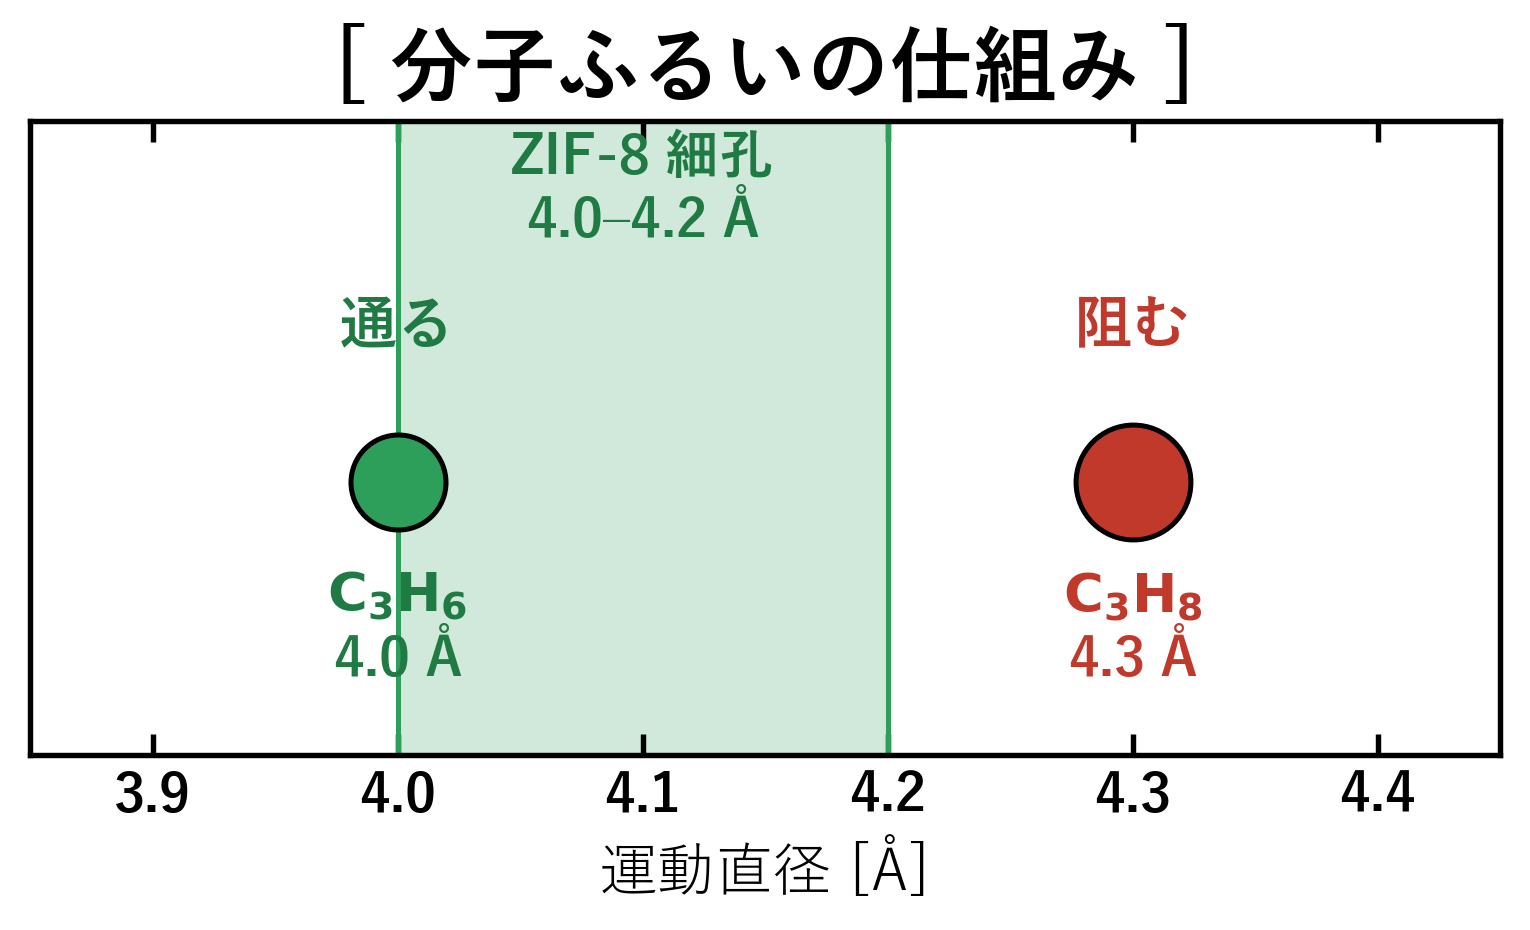
\includegraphics[width=0.99\linewidth]{sieving}\par
      \vspace{0.3em}
      \raggedright
      {\footnotesize\raggedright\linespread{1.16}\selectfont
       ZIF-8 のサブナノ細孔が運動直径差を識別。\par
       $\mathrm{C_3H_6}$ は透過・$\mathrm{C_3H_8}$ は阻止\par
       $\to$ 選択性 $\alpha=90$・透過度 $Q_A=40$ GPU\par}
      {\tiny\color{black!55} Hua et al., ACS Appl.\ Mater.\ Interfaces, \textbf{16}, 15273, 2024\par
       \vspace{0.2em}
       $1\,\mathrm{GPU}=3.35\times10^{-10}\ \mathrm{mol\,m^{-2}s^{-1}Pa^{-1}}$\par}
    \end{column}

    % ===== 右：モデル式（クロスフロー・溶解拡散）=====
    \begin{column}{0.61\textwidth}
      {\footnotesize\bfseries 推進力＝分圧差　線形透過則・溶解拡散}\par
      \vspace{0.12em}
      {\footnotesize\centering
       $\displaystyle J_{\mathrm{C_3H_6}} = Q_A\,(x P_H - y_{\mathrm{loc}} P_L)$\par
       \vspace{0.18em}
       $\displaystyle J_{\mathrm{C_3H_8}} = Q_B\,[(1-x) P_H - (1-y_{\mathrm{loc}}) P_L],\quad Q_B = Q_A/\alpha$\par}

      \vspace{0.42em}
      {\footnotesize\bfseries 物質収支　膜面積 $A$ 方向に積分}\par
      \vspace{0.12em}
      {\footnotesize\centering
       $\displaystyle \frac{dF_{\mathrm{C_3H_6}}}{dA} = -J_{\mathrm{C_3H_6}},\qquad
        \frac{dF_{\mathrm{C_3H_8}}}{dA} = -J_{\mathrm{C_3H_8}}$\par}

      \vspace{0.42em}
      {\footnotesize\bfseries 局所透過組成　クロスフロー　$\gamma = P_L/P_H$}\par
      \vspace{0.12em}
      {\footnotesize\centering
       $\displaystyle y_{\mathrm{loc}} = \frac{J_{\mathrm{C_3H_6}}}{J_{\mathrm{C_3H_6}}+J_{\mathrm{C_3H_8}}}$
       \quad$\to$\quad
       $(1-\alpha)\gamma\,y_{\mathrm{loc}}^2 + [(\alpha-1)(x+\gamma)+1]\,y_{\mathrm{loc}} - \alpha x = 0$\par}

      \vspace{0.45em}
      {\scriptsize\raggedright
       記号　$x$：非透過側 $\mathrm{C_3H_6}$ モル分率　$y_{\mathrm{loc}}$：局所透過組成　$P_H/P_L$：供給／透過側圧力　$A$：膜面積\par
       \vspace{0.15em}
       モジュール本数 $n=\lceil A_{\mathrm{mem}}/A_{\mathrm{module}}\rceil$、$A_{\mathrm{module}}=500\ \mathrm{m^2}$\par
       \vspace{0.15em}
       {\color{black!55} 前提：等温・等圧、透過度 $Q_A$・選択性 $\alpha$ は組成・圧力に非依存}\par}
    \end{column}
  \end{columns}

\end{frame}


\section{PSA原理1}
% =====================================================================
%  26  付録 PSA原理1 — 物理モデル。中央縦罫で左右2分割（スライド07/09に倣う）。
%   左＝物質収支の連立式（気相・固相LDF・吸着平衡）を説明付きで流す。
%   右＝活性炭の吸着パラメータ表とモデルの主要仮定。続く27でサイクル設計。
%  source_memo: 08_hydrogen_separation.tex §PSAカラムの物理モデル /
%   units/separators/psa/psa_system.py（PDE・LDF・Markham-Benton）/
%   src/cost_parameters.py（Langmuir 定数・KFa、Choi 2003・Rufford 2013）。
%  ルール：丸括弧禁止・最小色・[t] フレーム・帯と本文の重なり禁止。
% =====================================================================
\definecolor{SepGreen}{HTML}{2E9E5B}
\begin{frame}[t]

  \vspace*{2.4mm}
  % ===== 導入（全幅）。bold 行頭が帯へ近接するため上余白を確保 =====
  {\footnotesize\raggedright
   活性炭の固定床を\textbf{1 次元・等温・上流差分}でモデル化し、吸着成分
   \mbox{$\mathrm{CH_4}\!\cdot\!\mathrm{C_2H_4}\!\cdot\!\mathrm{C_2H_6}$} の濃度前線を時間発展で追う。\par}

  \vspace{0.55em}

  \begin{columns}[T,onlytextwidth]
    % ===== 左：物質収支の連立式（流す）=====
    \begin{column}{0.49\textwidth}
      {\bfseries 物質収支の連立}\par
      \vspace{0.5em}
      {\scriptsize 気相　対流の流入から固相へ移る分を差し引く}\par
      \vspace{0.15em}
      {\centering$\displaystyle
        \frac{\partial C_i}{\partial t}
          =-\frac{u_0}{\varepsilon}\frac{\partial C_i}{\partial z}
           -\frac{\rho_b}{\varepsilon}\frac{\partial q_i}{\partial t}$\par}
      \vspace{0.85em}
      {\scriptsize 固相 LDF　粒内拡散を平衡負荷との差の一次応答で近似}\par
      \vspace{0.15em}
      {\centering$\displaystyle \frac{\partial q_i}{\partial t}=K_F a_i\,(q_i^{*}-q_i)$\par}
      \vspace{0.85em}
      {\scriptsize 吸着平衡　多成分 Langmuir　Markham–Benton 形}\par
      \vspace{0.15em}
      {\centering$\displaystyle q_i^{*}=\frac{q_{s,i}\,a_i\,C_i}{1+\sum_j a_j C_j}$\par}
      \vspace{0.6em}
      {\scriptsize\color{black!55}\raggedright 競争吸着を表し、$\mathrm{C_2}$ 系ほど親和定数 $a$ が大きい。\par}
    \end{column}

    % ===== 中央：全高の仕切り線 =====
    \begin{column}{0.02\textwidth}
      \centering
      {\color{black!35}\rule[-6.0cm]{0.6pt}{6.2cm}}
    \end{column}

    % ===== 右：パラメータ表＋主要仮定 =====
    \begin{column}{0.49\textwidth}
      {\bfseries 吸着パラメータ　活性炭 $25\,^\circ$C}\par
      \vspace{0.5em}
      {\centering
       {\footnotesize\renewcommand{\arraystretch}{1.12}\setlength{\tabcolsep}{6pt}%
        \begin{tabular}{@{}l c c c@{}}
          \toprule
          成分 & $q_{s}$ & $a$ & $K_F a$ \\
                & {\scriptsize mol/kg} & {\scriptsize m$^3$/mol} & {\scriptsize 1/s} \\
          \midrule
          $\mathrm{CH_4}$   & $5.23$ & $3.32\!\times\!10^{-3}$ & $0.020$ \\
          $\mathrm{C_2H_4}$ & $6.20$ & $3.27\!\times\!10^{-2}$ & $0.015$ \\
          $\mathrm{C_2H_6}$ & $5.66$ & $5.33\!\times\!10^{-2}$ & $0.011$ \\
          \bottomrule
        \end{tabular}}\par}
      \vspace{0.3em}
      {\scriptsize\color{black!55}\raggedright 等温線 Choi \textit{et al.}, 2003／移動係数 Rufford \textit{et al.}, 2013\par}
      \vspace{0.85em}
      {\bfseries 主要仮定}\par
      \vspace{0.3em}
      {\footnotesize\raggedright\linespread{1.22}\selectfont
        $\bullet$ \textbf{\color{SepGreen!45!black}水素は非吸着}　全量を製品へ\par
        \vspace{0.22em}
        $\bullet$ $\mathrm{C_3}$ は入口で即時吸着　全量オフガスへ\par
        \vspace{0.22em}
        $\bullet$ 吸着 PDE は上記 3 成分のみで解く\par
        \vspace{0.22em}
        $\bullet$ 破過は $\mathrm{CH_4}$ 出口が入口の $0.1$\%\par}
    \end{column}
  \end{columns}

\end{frame}


\section{PSA原理2}
% =====================================================================
%  27  付録 PSA原理2 — サイクル設計。中央縦罫で左右2分割（26と統一、07/09に倣う）。
%   左＝吸着工程（破過→周期定常補正）／右＝脱着工程と必要塔数。
%   下に全幅の結論帯（型F「結論を枠で締める」）。説明を添えて式を流す。
%  source_memo: 08_hydrogen_separation.tex §脱着工程の簡易モデル/周期定常状態の
%   簡易補正/スイングサイクルと塔数の決定 / units/separators/psa/psa_system.py。
%  ルール：丸括弧禁止・最小色・[t] フレーム・帯と本文の重なり禁止。
% =====================================================================
\begin{frame}[t]

  \vspace*{2.4mm}
  % ===== 導入（全幅）。bold 行頭が帯へ近接するため上余白を確保 =====
  {\footnotesize\raggedright
   バッチの吸着・脱着を\textbf{複数塔の位相をずらして並列運転}し連続供給に変える。
   各工程の所要時間と必要塔数を次の順で決める。\par}

  \vspace{0.55em}

  \begin{columns}[T,onlytextwidth]
    % ===== 左：吸着工程 =====
    \begin{column}{0.49\textwidth}
      {\bfseries 吸着工程}\par
      \vspace{0.5em}
      {\footnotesize\bfseries 破過まで}\par
      \vspace{0.1em}
      {\scriptsize\raggedright PDE を解き、$\mathrm{CH_4}$ 出口が入口の $0.1$\% に達した時刻を清浄床の破過時間 $t_{\mathrm{abs,clean}}$ とする。\par}
      \vspace{0.85em}
      {\footnotesize\bfseries 周期定常補正}\par
      \vspace{0.1em}
      {\scriptsize\raggedright 前サイクルの残留を基準 ${\color{SpRed}\beta}$ 相当と見込み、吸着時間を短く補正する保守側の扱い。\par}
      \vspace{0.3em}
      {\centering$\displaystyle t_{\mathrm{abs}}\approx t_{\mathrm{abs,clean}}\,(1-{\color{SpRed}\beta})$\par}
      \vspace{0.7em}
      {\scriptsize\color{black!55}\raggedright 床全体に基準 ${\color{SpRed}\beta}$ 相当の残留が一様にあるとみなし、清浄床の破過時刻から補正する。残留を過大評価し塔数を多めに見積もる向き。\par}
    \end{column}

    % ===== 中央：仕切り線 =====
    \begin{column}{0.02\textwidth}
      \centering
      {\color{black!35}\rule[-4.4cm]{0.6pt}{4.6cm}}
    \end{column}

    % ===== 右：脱着工程と必要塔数 =====
    \begin{column}{0.49\textwidth}
      {\bfseries 脱着工程と必要塔数}\par
      \vspace{0.5em}
      {\footnotesize\bfseries 脱着}\quad{\scriptsize 低圧パージで $q^{*}\!\approx\!0$、指数減衰}\par
      \vspace{0.15em}
      {\centering$\displaystyle q_i(t)=q_{i,0}\,\exp(-K_F a_i\,t)$\par}
      \vspace{0.2em}
      {\scriptsize\raggedright 残量比が ${\color{SpRed}\beta}$ に達するまでが $t_{\mathrm{des}}$、安全係数 $1.2$ を乗じる\par}
      \vspace{0.15em}
      {\centering$\displaystyle \sum_i q_i(t_{\mathrm{des}})\Big/\sum_i q_{i,0}={\color{SpRed}\beta}$\par}
      \vspace{0.7em}
      {\footnotesize\bfseries 必要塔数}\quad{\scriptsize 残塔が脱着を終える本数＋予備 1}\par
      \vspace{0.15em}
      {\centering$\displaystyle N_{\mathrm{cycle}}=\left\lceil t_{\mathrm{des}}/t_{\mathrm{abs}}\right\rceil+1$\par}
      \vspace{0.12em}
      {\centering$\displaystyle N_{\mathrm{total}}=N_{\mathrm{par}}\times N_{\mathrm{cycle}}$\par}
    \end{column}
  \end{columns}

  \vspace{0.7em}
  % ===== 全幅：結論帯 ＋ 仮定注記 =====
  {\setlength{\fboxsep}{6pt}%
   \noindent\colorbox{HiBlue!22}{%
    \begin{minipage}{\dimexpr\linewidth-2\fboxsep\relax}
     {\footnotesize 本設計は $N_{\mathrm{par}}{=}1$、$t_{\mathrm{des}}\!\ll\!t_{\mathrm{abs}}$ ゆえ
      \textbf{吸着 1 塔・脱着 1 塔の計 2 塔}で連続供給が成立する。\par}
    \end{minipage}}}
  \vspace{0.35em}
  {\scriptsize\color{black!55}\raggedright 等温・等速は塔数を多めに見積もる保守側の近似。水素回収率はサイクル簡略化により暫定。\par}

\end{frame}


\section{PSA検証}
% =====================================================================
%  27  付録 PSA検証 — 骨格（スライド3と同じく現状は意図的に空白）
%  source_memo 候補: exp/exp_psa_sensitivity.py（吸着材データ不確かさの感度：
%   KFa×0.5/2.0・q_s±30%・a±50%・rho_b 400/600/700 で 塔数・H2回収率・TAC の頑健性）
%   ＋bin/tests/test_css_approximation.py・test_h2_loss_purge.py（CSS 近似・H2 損失検証）。
%  ルール：丸括弧禁止・最小色・[t] フレーム・帯と本文の重なり禁止。
% =====================================================================
\begin{frame}[t]

  % ↓↓↓ 中身ができたらここに置く ↓↓↓

\end{frame}


\section{発熱材}
% =====================================================================
%  28  付録 HGM — 骨格（スライド3と同じく現状は意図的に空白）
%  source_memo 候補: 04_reaction.tex の HGM モデル（床温下限 T_in−ΔT_max、
%   ΔT_max=50 K・φ_cat=0.85）＋tools/build_hgm_sensitivity_nb.py
%   （ΔT_max=30/50/80 K 感度：X・生産量・TAC への効き）。
%  ルール：丸括弧禁止・最小色・[t] フレーム・帯と本文の重なり禁止。
% =====================================================================
\begin{frame}[t]

  % ↓↓↓ 中身ができたらここに置く ↓↓↓

\end{frame}


\section{TPE}
% =====================================================================
%  30  付録 TPE／Optuna — 中央縦罫で左右2分割（26/27 に統一）。
%   左＝TPE アルゴリズムの要点（良/悪2群への分割・l/g 比の取得規準・名称の2性質）。
%   右＝Optuna による実装（多変量TPE・Sobol起動・制約信号25・SQLite再開/並列）。
%  source_memo: 10/11_optimization.tex＋optimization/study.py
%   （multivariate TPE・QMC Sobol 50 起動・constraints_func 25 信号・SQLite 再開・constant_liar 並列）。
%   一般説明は Bergstra 2011／Optuna TPESampler ドキュメント。
%  ルール：丸括弧禁止・最小色・[t] フレーム・帯と本文の重なり禁止。左は簡潔に要点のみ。
% =====================================================================
\begin{frame}[t]

  \vspace*{2.4mm}

  \begin{columns}[T,onlytextwidth]
    % ===== 左：TPE アルゴリズムの要点 =====
    \begin{column}{0.49\textwidth}
      {\small\bfseries TPE}\;{\scriptsize Tree-structured Parzen Estimator}\par
      \vspace{0.5em}
      {\scriptsize\raggedright 評価コストの高いブラックボックス最小化
        \mbox{$x^{\star}=\arg\min_{x}f(x)$} を、過去の観測から次の評価点を提案する
        逐次モデルベース最適化として解く。ガウス過程が $p(y\mid x)$ を直接モデル化するのに対し、
        \textbf{TPE は条件を反転して $p(x\mid y)$ を推定する}。\par}
      \vspace{0.6em}
      {\scriptsize\bfseries 観測を良群・悪群に二分}\par
      \vspace{0.2em}
      {\scriptsize\raggedright 目的値の $\gamma$ 分位点を閾値 $y^{\star}$
        \mbox{$P(y<y^{\star})={\color{SpRed}\gamma}$} とし、各群で $x$ の条件付き密度を構成する。\par}
      \vspace{0.3em}
      {\centering\resizebox{0.96\linewidth}{!}{$
        l(x)=p(x\mid y<y^{\star}),\quad
        g(x)=p(x\mid y\ge y^{\star})$}\par}
      \vspace{0.55em}
      {\scriptsize\bfseries 取得規準}\par
      \vspace{0.15em}
      {\centering\boldmath$\displaystyle
        x_{\mathrm{next}}=\arg\max_{x}\,\frac{l(x)}{g(x)}$\unboldmath\par}
      \vspace{0.3em}
      {\scriptsize\raggedright 良群で密・悪群で疎な領域を選ぶ操作で、期待改善 EI の最大化と等価。\par}
      \vspace{0.55em}
      {\scriptsize\bfseries 名称が表す2つの性質}\par
      \vspace{0.15em}
      {\scriptsize\raggedright
        \textbf{Parzen}　密度 $l,g$ をカーネル密度推定で近似する。\par
        \vspace{0.25em}
        \textbf{Tree-structured}　条件で有効変数が変わる木構造の探索空間を扱い、混合変数に強い。\par}
    \end{column}

    % ===== 中央：全高の仕切り線 =====
    \begin{column}{0.02\textwidth}
      \centering
      {\color{black!35}\rule[-6.5cm]{0.6pt}{6.7cm}}
    \end{column}

    % ===== 右：Optuna による実装 =====
    \begin{column}{0.49\textwidth}
      {\small\bfseries Optuna}\;{\scriptsize による実装}\par
      \vspace{0.5em}
      {\scriptsize\raggedright TPE を実装したベイズ最適化フレームワーク。
        罰則を加えた年経費 TAC を目的関数とし、最小化方向で探索する。\par}
      \vspace{0.6em}
      {\scriptsize\bfseries 多変量 TPE}\par
      \vspace{0.1em}
      {\scriptsize\raggedright 密度 $l,g$ を多変量化し、変数間の相関を学習する。
        変数ごとに独立な密度推定では捉えられない。\par}
      \vspace{0.5em}
      {\scriptsize\bfseries 2 段サンプリング}\par
      \vspace{0.1em}
      {\scriptsize\raggedright 初期 $50$ 点を Sobol 列の準モンテカルロで広く撒き、
        以降 TPE に切替える。狭い実行可能領域を取りこぼしにくい。\par}
      \vspace{0.5em}
      {\scriptsize\bfseries 制約情報の受け渡し}\par
      \vspace{0.1em}
      {\scriptsize\raggedright $25$ 本の制約信号を
        \mbox{負＝実行可能・正＝違反} として渡し、TPE が実行可能解と違反解を分けて学習する。\par}
      \vspace{0.5em}
      {\scriptsize\bfseries 運用機能}\par
      \vspace{0.1em}
      {\scriptsize\raggedright 履歴を SQLite に保存して中断・再開でき、並列実行にも対応する。\par}
    \end{column}
  \end{columns}

\end{frame}


\end{document}
